\chapter{\uppercase{Neutrino Oscillation in the PROSPECT AD}}

\section{Detecting Antineutrinos}

PROSPECT detects $\bar{\nu_e}$'s via the inverse beta decay reaction (IBD):
\begin{equation}
	\bar{\nu_e} + p \rightarrow e^+ + n
\end{equation}
A reactor $\bar{\nu_e}$ will interact with a proton in the $^6$Li-LS, producing a positron and a neutron.
The positron will quickly lose energy and annihilate with an electron, producing two 511 keV $\gamma$-rays.
This is the prompt signal.

Concurrently, the neutron will thermalize by scattering off of protons in the scintillator until it captures on $^6$Li ($\sim$80\% of the time) or H ($\sim$20\% of the time).
The neutron capture on $^6$Li (nLi) produces a tritium and an alpha with energies 2.05 MeV and 2.75 MeV respectively. 
These two products will immediately scintillate, and produce a quenched signal of $\sim$0.55 MeVee.
This is the delayed signal.
Figure~\ref{fig:ibd} illustrates this process in the PROSPECT LiLS.

The neutron capture on $^6$Li takes $\sim$40$\mu$s, providing a time separation between the prompt and delayed signals.
Making use of the time coincident, PSD, and energy cuts, PROSPECT can identify $\bar{\nu_e}$ events above background. 

\begin{figure}[!t]
	\centering
	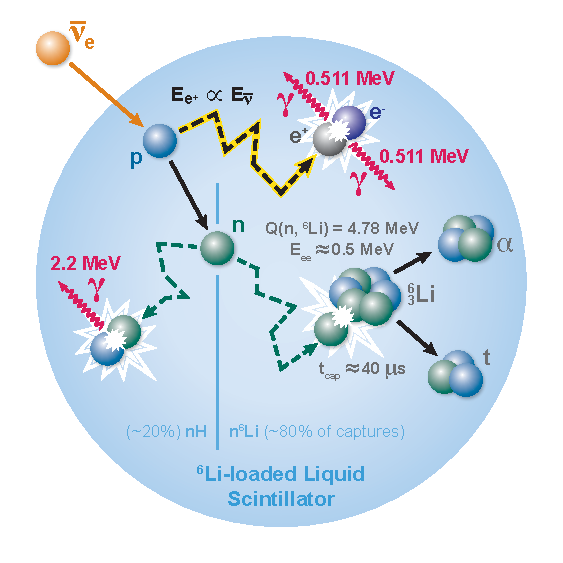
\includegraphics[width=0.4\linewidth]{tex/7-oscillation-images/IBD}
	\caption{Schematic of the IBD interaction is the PROSPECT AD.}
	\label{fig:ibd}
\end{figure}

\section{IBD Event Selection}

\subsection{Cuts}

A selection of energy, PSD, and time cuts, along with specified event vetos are utilized to identify IBD signals and reduce background.
These are:
\begin{itemize}
	\item Prompt Cluster Size: $\geq1$
	\item Prompt PSD: All pulses must have PSD that is $<3\sigma$ from the gamma-like PSD band mean
	\item Prompt Energy: No cut, but only clusters with a total energy of 0.8 $<$ E$_{\textrm{rec}} <$ 7.2 MeV are used in the oscillation analysis
	\item Delayed Cluster Size: Single pulse
	\item Delayed PSD: All pulses must have PSD that is $>3.6\sigma$ from the gamma-like PSD band mean
	\item Delayed Energy: 0.46 $<$ E$_{\textrm{rec}} < $0.60 MeV
	\item Time Correlation: $\Delta t = (1,120)~\mu$s
	\item Prompt-Delayed Distance: $\Delta z <$ 18 cm for coincidences in the same segment; $\Delta z <$ 14 cm for coincidences in horizontally/vertically adjacent segments
	\item Pileup Veto: Applied to both prompt and delayed clusters, if the candidate cluster is preceded by another cluster in a window of $<$ 800 ns, the candidate cluster is vetoed
	\item Shower Veto: Veto delayed clusters that exist in a (0,100) $\mu$s window around cosmic muon clusters (E$_{\textrm{rec}} >$ 15 MeV); Veto delayed clusters that exist within (-200,+200)~$\mu$s of events with PSD $> 3\sigma$ from the gamma-like PSD band mean and E $>$ 0.25 MeV
	\item Fiducialization: Reject events in which a prompt or delayed event occurs in the outer ring of segments; reject events that occur outside of $z$ = (-448, 448) mm 
\end{itemize}
For an example of how the PSD and energy cuts look in PSD versus energy space for prompt events correlated with a delayed neutron capture see Figure~\ref{fig:psdvsecorrnli}.

\begin{figure}[h]
	\centering
	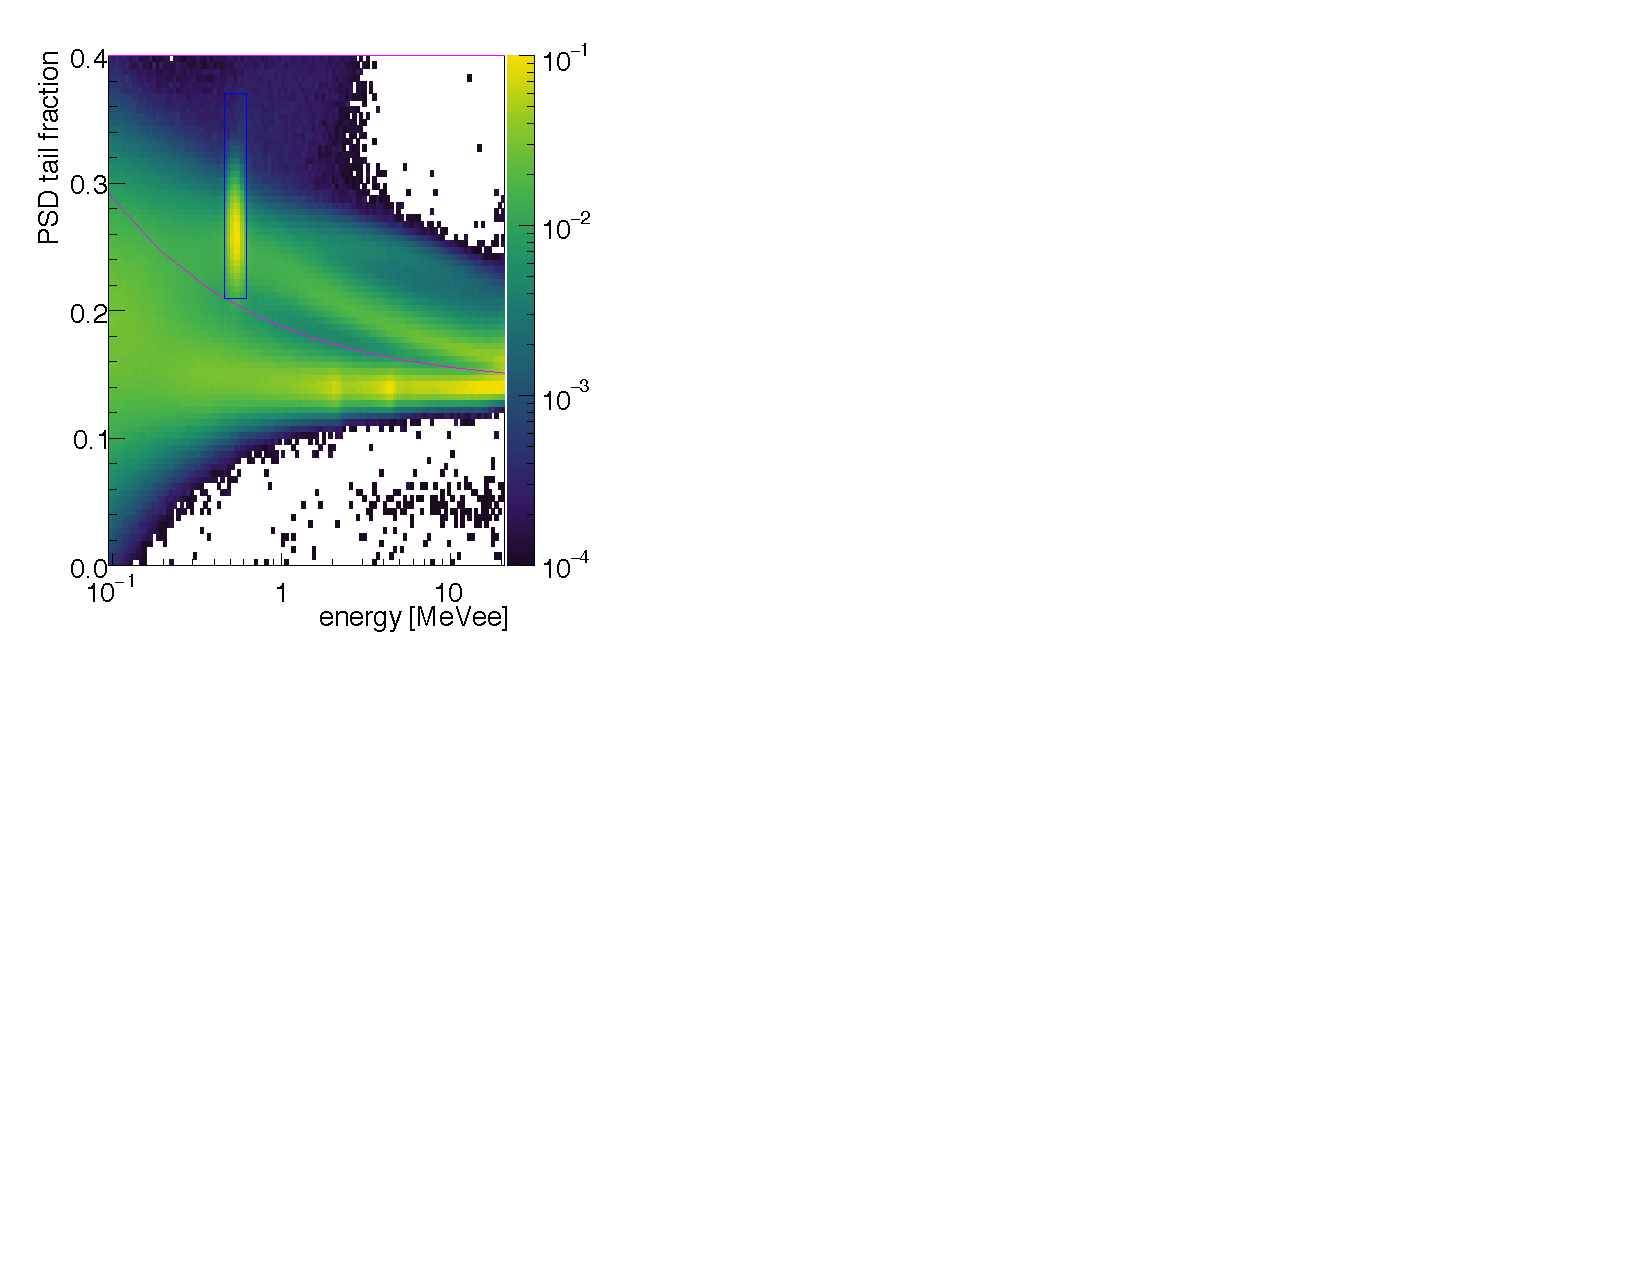
\includegraphics[width=0.6\linewidth]{tex/7-oscillation-images/PSDvsE_Corr_nLi}
	\caption{PSD versus energy distribution for prompt events correlated with a delayed neutron capture on $^6$Li. The cuts used for identifying nLi events is represented by the blue rectangle. The upper limit of the cut used for identifying electron-like signals is shown as the pink curve.}
	\label{fig:psdvsecorrnli}
\end{figure}



\subsection{Backgrounds}

The two primary backgrounds to the IBD signal are time-correlated cosmogenic neutron events and accidental coincidences of ambient $\gamma$-rays and nLi captures.
Cosmic muons moving through the lead shielding can create multiple neutrons that may be selected as delayed events.
The shower veto helps to reduce this background, introducing a dead-time that varies between 5.5\% and 6.9\% for reactor off and on times respectively.
Along with this veto, the IBD selection is applied to reactor off data and the resulting distributions are subtracted from the reactor on results.

Accidental coincidences are handled by selecting prompt-delay pairs with $\Delta t$ = (-12,-2) ms.
This provides a high statistics sample of events that are scaled to match the correlated time window and then subtracted from the correlated events. 
This is done for both reactor on and off data sets.

\begin{figure}[!b]
	\centering
	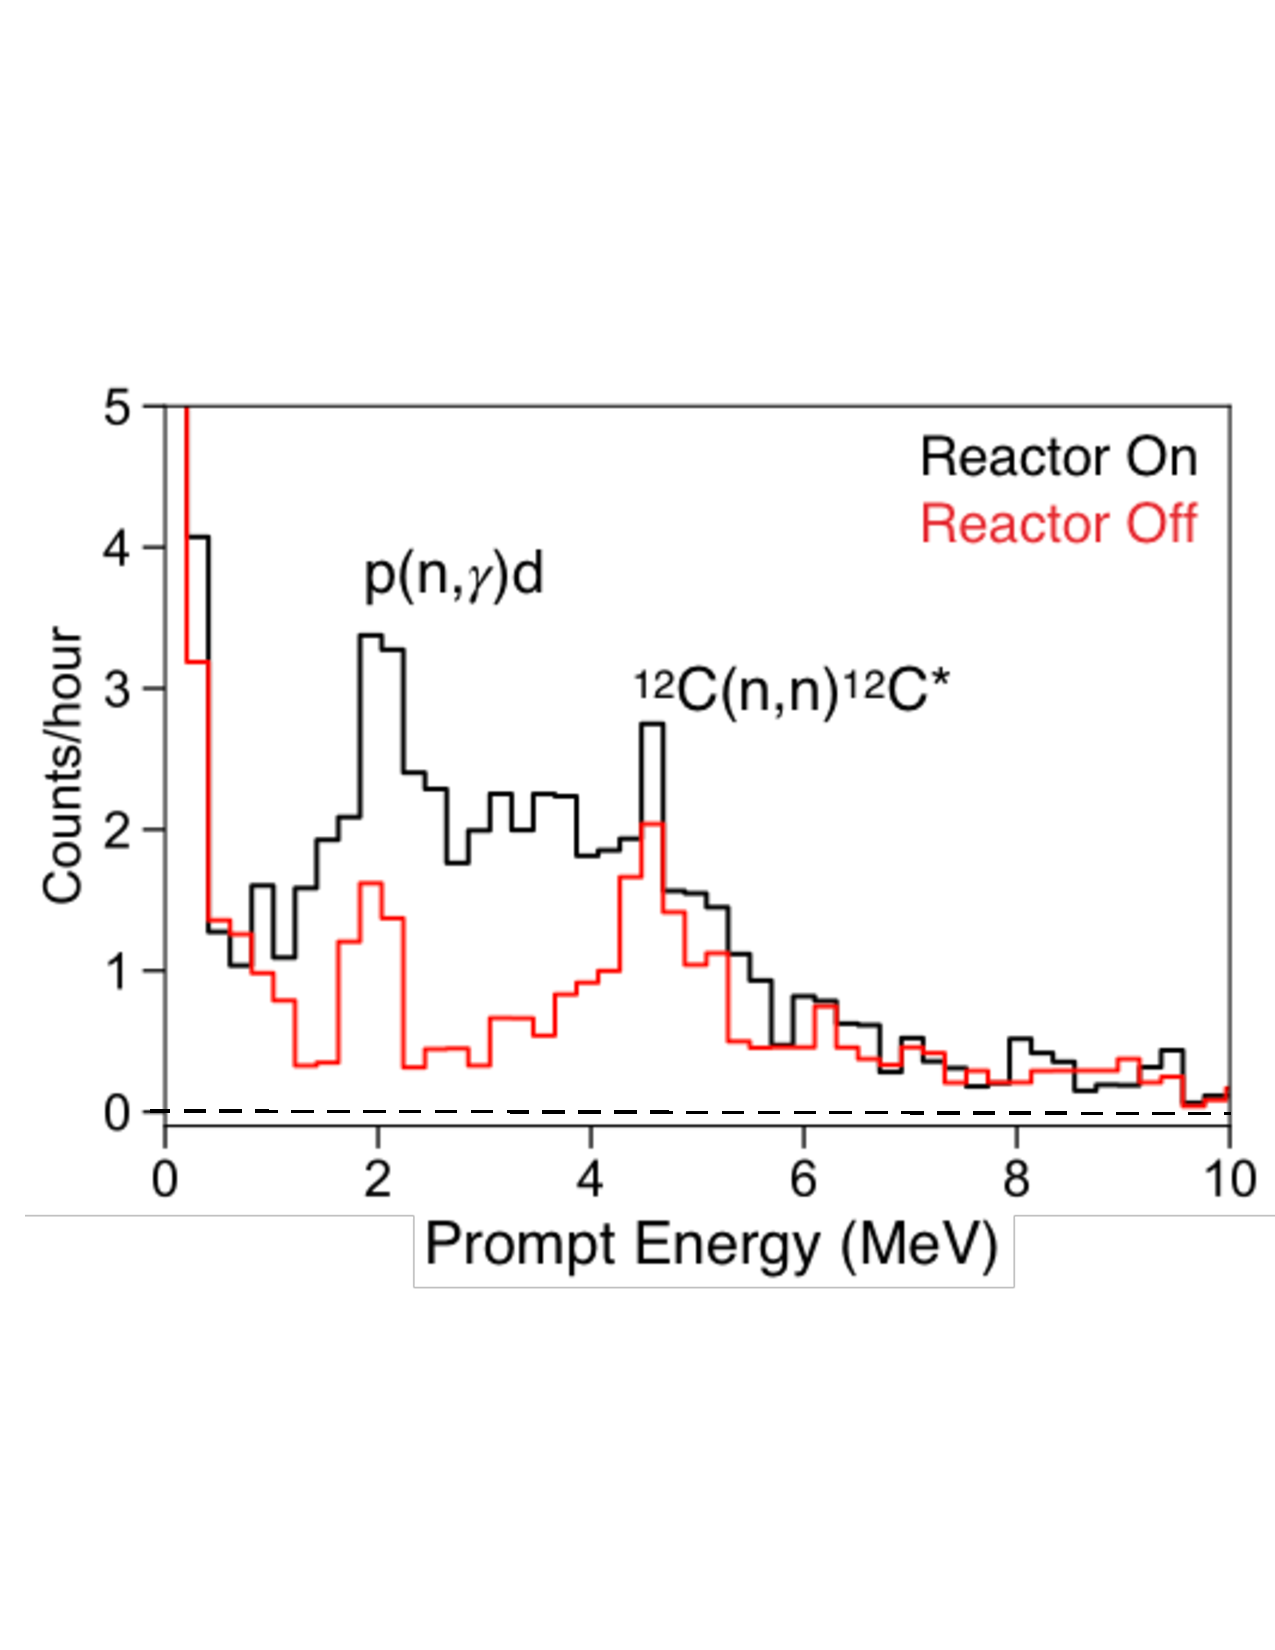
\includegraphics[width=0.6\linewidth]{tex/7-oscillation-images/IBD_E}
	\caption{The prompt energy spectra, after background subtraction, of IBD events for 24 hours of both reactor on and off data. Prominent peaks at 2.2 MeV and 4.4 MeV are due to neutron captures on Hydrogen and inelastic neutron scatters on $^{12}$C respectively.}
	\label{fig:ibde}
\end{figure}

Figure~\ref{fig:ibde} shows the prompt energy spectra for 24 hours both of reactor on and off data after applying all cuts and accidental background subtraction.
Prominent peaks at 2.2 MeV and 4.4 MeV exist in both reactor on and off data.
Cosmogenic muons can create several neutrons. One of these will capture on hydrogen (nH), producing a 2.2 MeV $\gamma$, which will be followed by another neutron capturing on $^6$Li. 
These time-coincident events are reduced by the shower veto, but not completely removed.

Fast neutrons will also inelastically scatter off of $^{12}$C in the scintillator causing the reaction:
\begin{equation}
	n + ^{12}C \rightarrow n' + ^{12}C^*
\end{equation}
As $^{12}$C$^*$ de-excites it will release a 4.4 MeV photon, while the scattered neutron thermalizes and captures on $^{6}$Li, mimicking the IBD signal.


\subsection{Atmospheric Correction}

Cosmogenic rates vary according to changes in pressure, therefore, a scaling factor for this effect needs to be introduced in order to perform accurate background subtraction.
To determine the size of this correction fast neutron events with a prompt proton recoil and a delayed nLi capture (FN+nLi) were studied. 
The prompt event was required to have PSD $>3\sigma$ from the gamma-like PSD band mean, otherwise all other cuts used were the same as the ones used for IBD selection.

\begin{figure}[!b]
	\begin{subfigure}{0.5\linewidth}
		\centering
		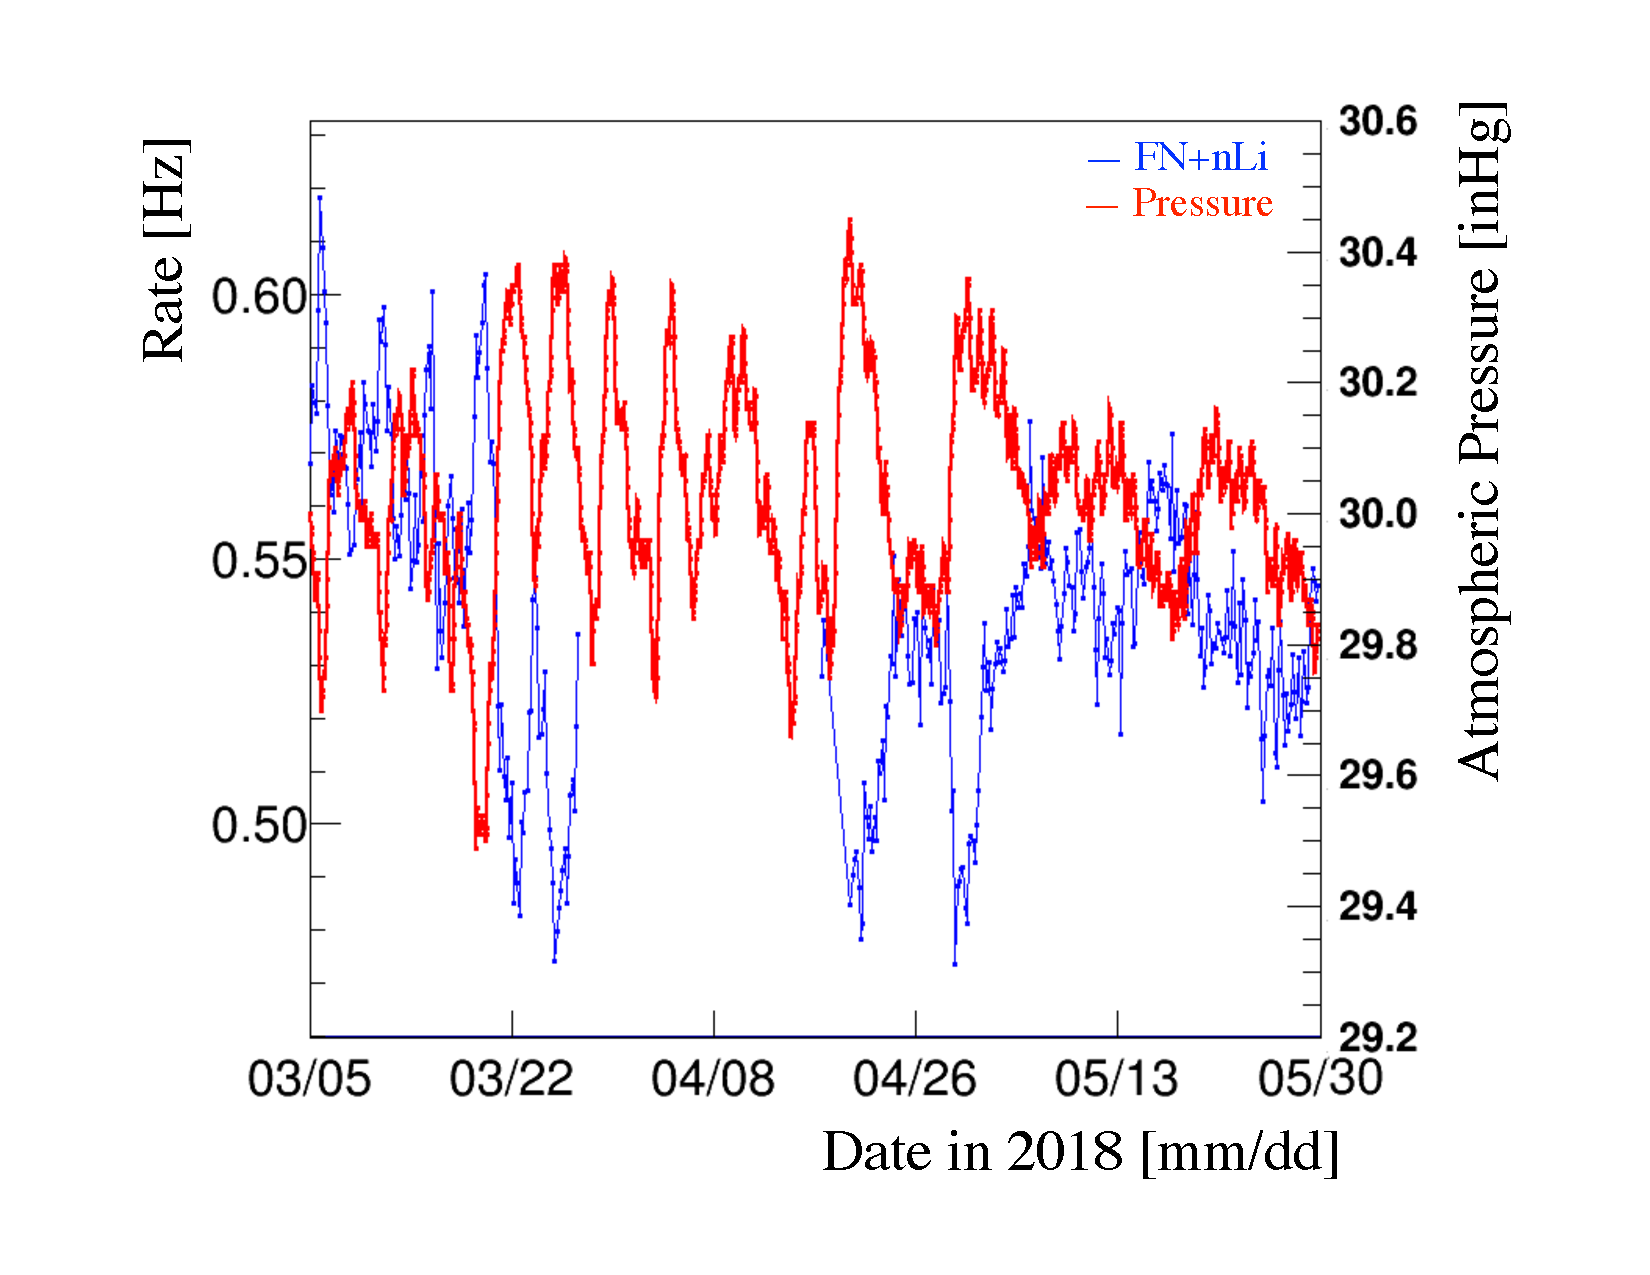
\includegraphics[width=0.95\linewidth]{tex/7-oscillation-images/FNnLi_Rate}
		%\caption{}
		\label{fig:fnnlirate}
	\end{subfigure}
	\begin{subfigure}{0.5\linewidth}
		\centering
		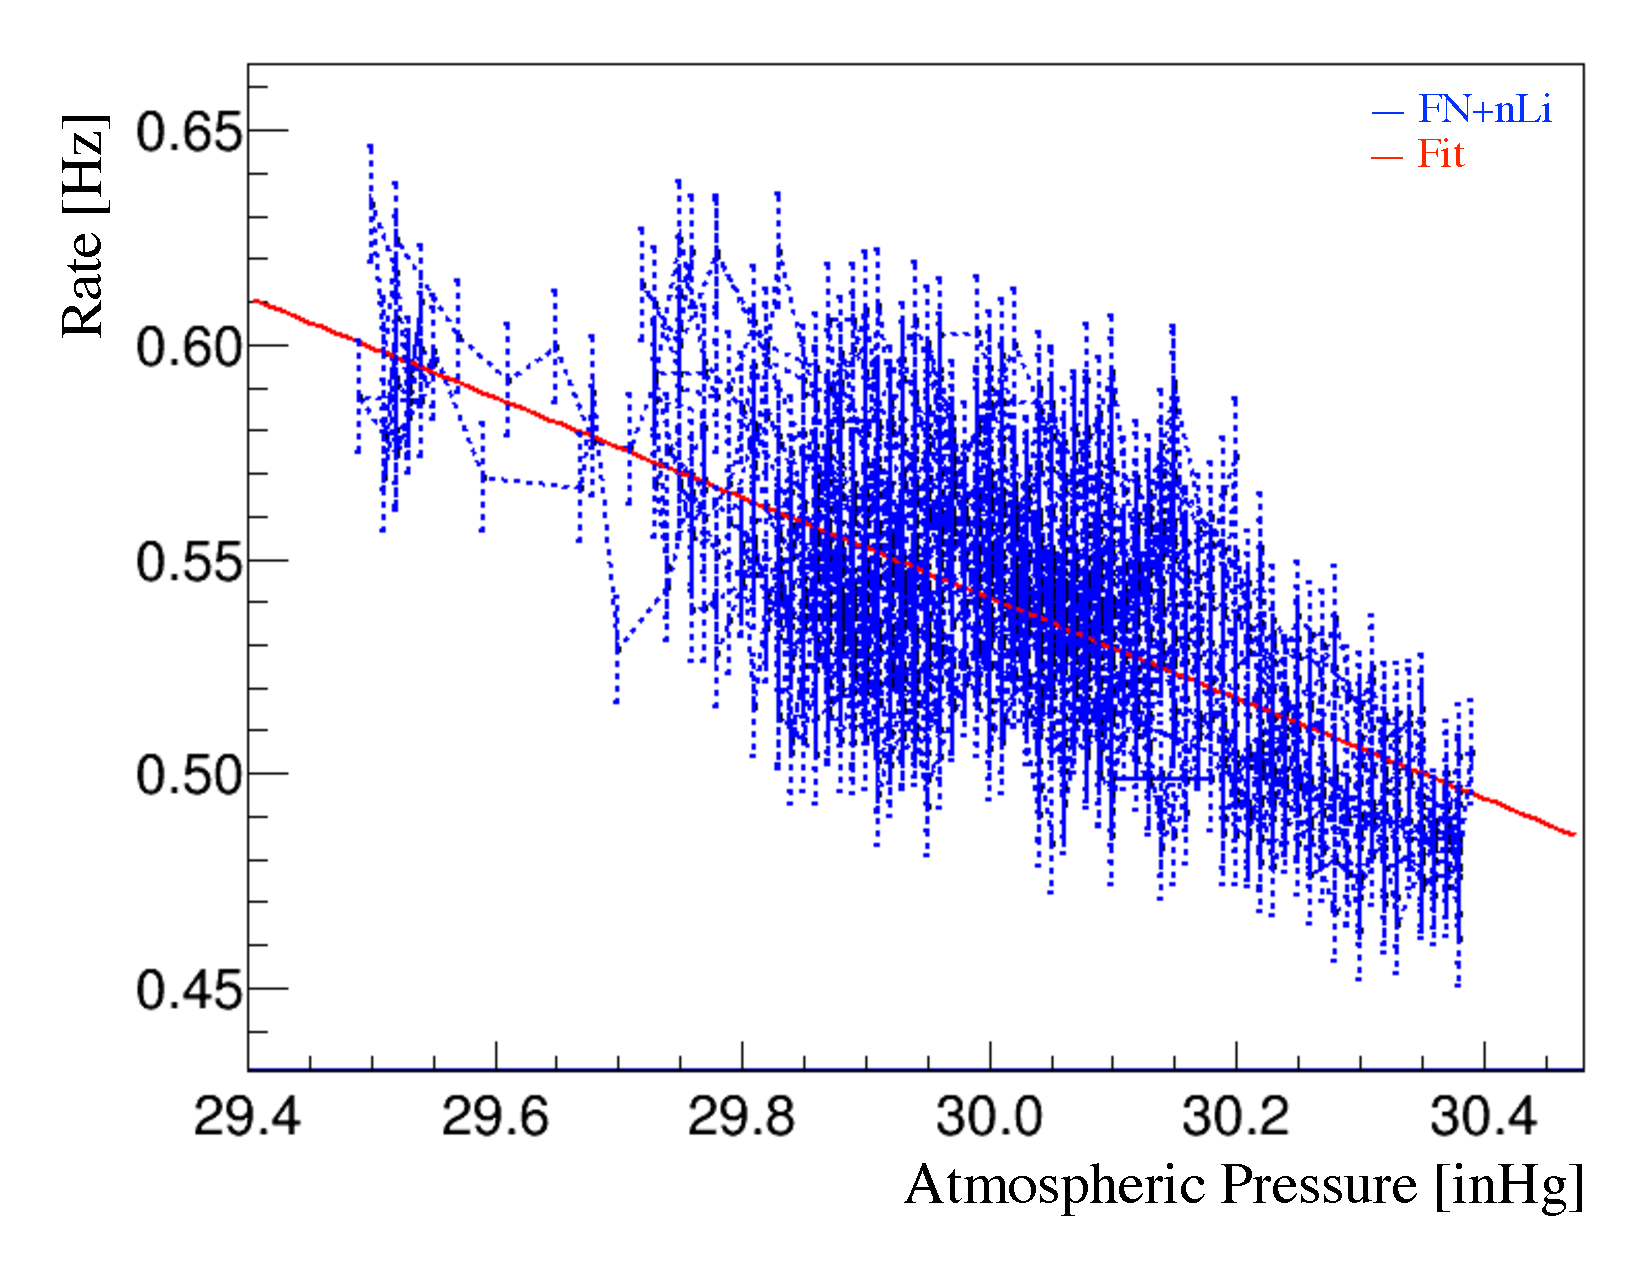
\includegraphics[width=0.95\linewidth]{tex/7-oscillation-images/FNnLi_RateVsPressure}
		%\caption{}
		\label{fig:fnnliratevspressure}
	\end{subfigure}
	\caption[]{(Left) The rate of fast neutron and nLi capture coincidences (blue) and pressure (red) versus time. (Right) FN+nLi rates as a function of pressure with a linear fit. \cite{Kyzylova2370:2018}}
	\label{fig:atm}
\end{figure}


Figure~\ref{fig:atm} shows the rate of these coincident events and pressure versus time, along with rate versus pressure.
It can be seen that the event rate and pressure are inversely correlated. 
The rate of FN+nLi events as a function of pressure was fit with a linear function and the results of the fit were used to define the atmospheric correction, $k_p$, according to
\begin{equation}
k_p = \frac{m \cdot \bar{p}_{on} + c}{m \cdot \bar{p}_{off} + c}
\end{equation}
where $m$ and $c$ are the slope and y-intercept of the fit and $\bar{p}_{on (off)}$ is the average pressure during reactor on (off).
For this analysis the atmospheric correction was found to be $<$ 1\%.


\subsection{Background Subtraction}

To obtain the final measured IBD events the correlated and accidental events are subtracted for both reactor on and off time periods.
Due to differences in reactor on and off exposure time, as well as differences between accidental and coincidental acceptance time windows, accidental and reactor off events have to be correctly scaled.
Therefore, the number of IBD candidates, $N_{IBD}$, is measured as:
\begin{equation}
\begin{split}
	N_{IBD} &= N_{corr-acc, on} - k_p \cdot N_{corr-acc, off} \\
				 &= N_{corr, on} - \frac{\Delta t_{corr}}{\Delta t_{acc}} N_{acc, on} - k_p \frac{t_{on}}{t_{off}}\left(N_{corr, off} - \frac{\Delta t_{corr}}{\Delta t_{acc}}N_{acc,off}\right)
\end{split}
\end{equation}


\section{Data Set}

The dataset used in this analysis consists of 30.26 (33) reactor on and 26.19 (28) reactor off effective (calendar) days.
The rate of correlated and accidental rates for each of these periods are listed in Table~\ref{tab:datastats}.
A total of 25461 IBD events were detected (771/day), with a signal-to-background ratio of 2.20 and 1.32 for accidental and correlated background, respectively.
The correlated and accidental rates per day as a function of time for events in the prompt energy region (0.8, 7.2) MeV can be seen in Figure~\ref{fig:evtrates}.

Due to current instabilities observed in some PMT's during the data-taking period 31 segments were excluded in this analysis: (0, 1, 2, 3, 4, 5, 6, 9, 10, 11, 12, 13, 18, 21, 23, 24, 27, 32, 34, 40, 44, 52, 68, 79, 86, 102, 115, 122, 127, 130, 139).
Two segments not in the outer shell were also added to the non-fiducial volume due to high background rates: (25, 26).
These two segments exist in a corner of the detector that does not sit on the monolith and therefore they see many $\gamma$-rays from beam lines under the floor.

\begin{table}[H]
\begin{tabular}{|c|c|c|c|}
	\hline 
	\textbf{Reactor} & \textbf{Event Type} & \textbf{Time [days]} & \textbf{Counts} \\ 
	\hline 
	& Correlated + Accidental &  & 56378 $\pm$ 1708 \\ 
	On & Accidental (scaled) & 30.26 & 11580 $\pm$ 12 \\ 
	& Correlated &  & 44797 $\pm$ 238 \\ 
	\hline 
	& Correlated + Accidental (scaled) & & 20262 $\pm$ 153   \\ 
	Off &  Accidental (scaled) & 26.19  & 925 $\pm$ 4   \\ 
	& Correlated (scaled) & & 19337 $\pm$ 153 \\ 
	\hline 
	\hline 
	& Signal &  & 25461 $\pm$ 238 (771/day) \\ 
	\hline 
\end{tabular} 
\caption{The total number of correlated and accidental events in the prompt energy region (0.8, 7.2) MeV for reactor on and off periods. Time refers to exposure time.}
\label{tab:datastats}
\end{table}

\begin{figure}[H]
	\centering
	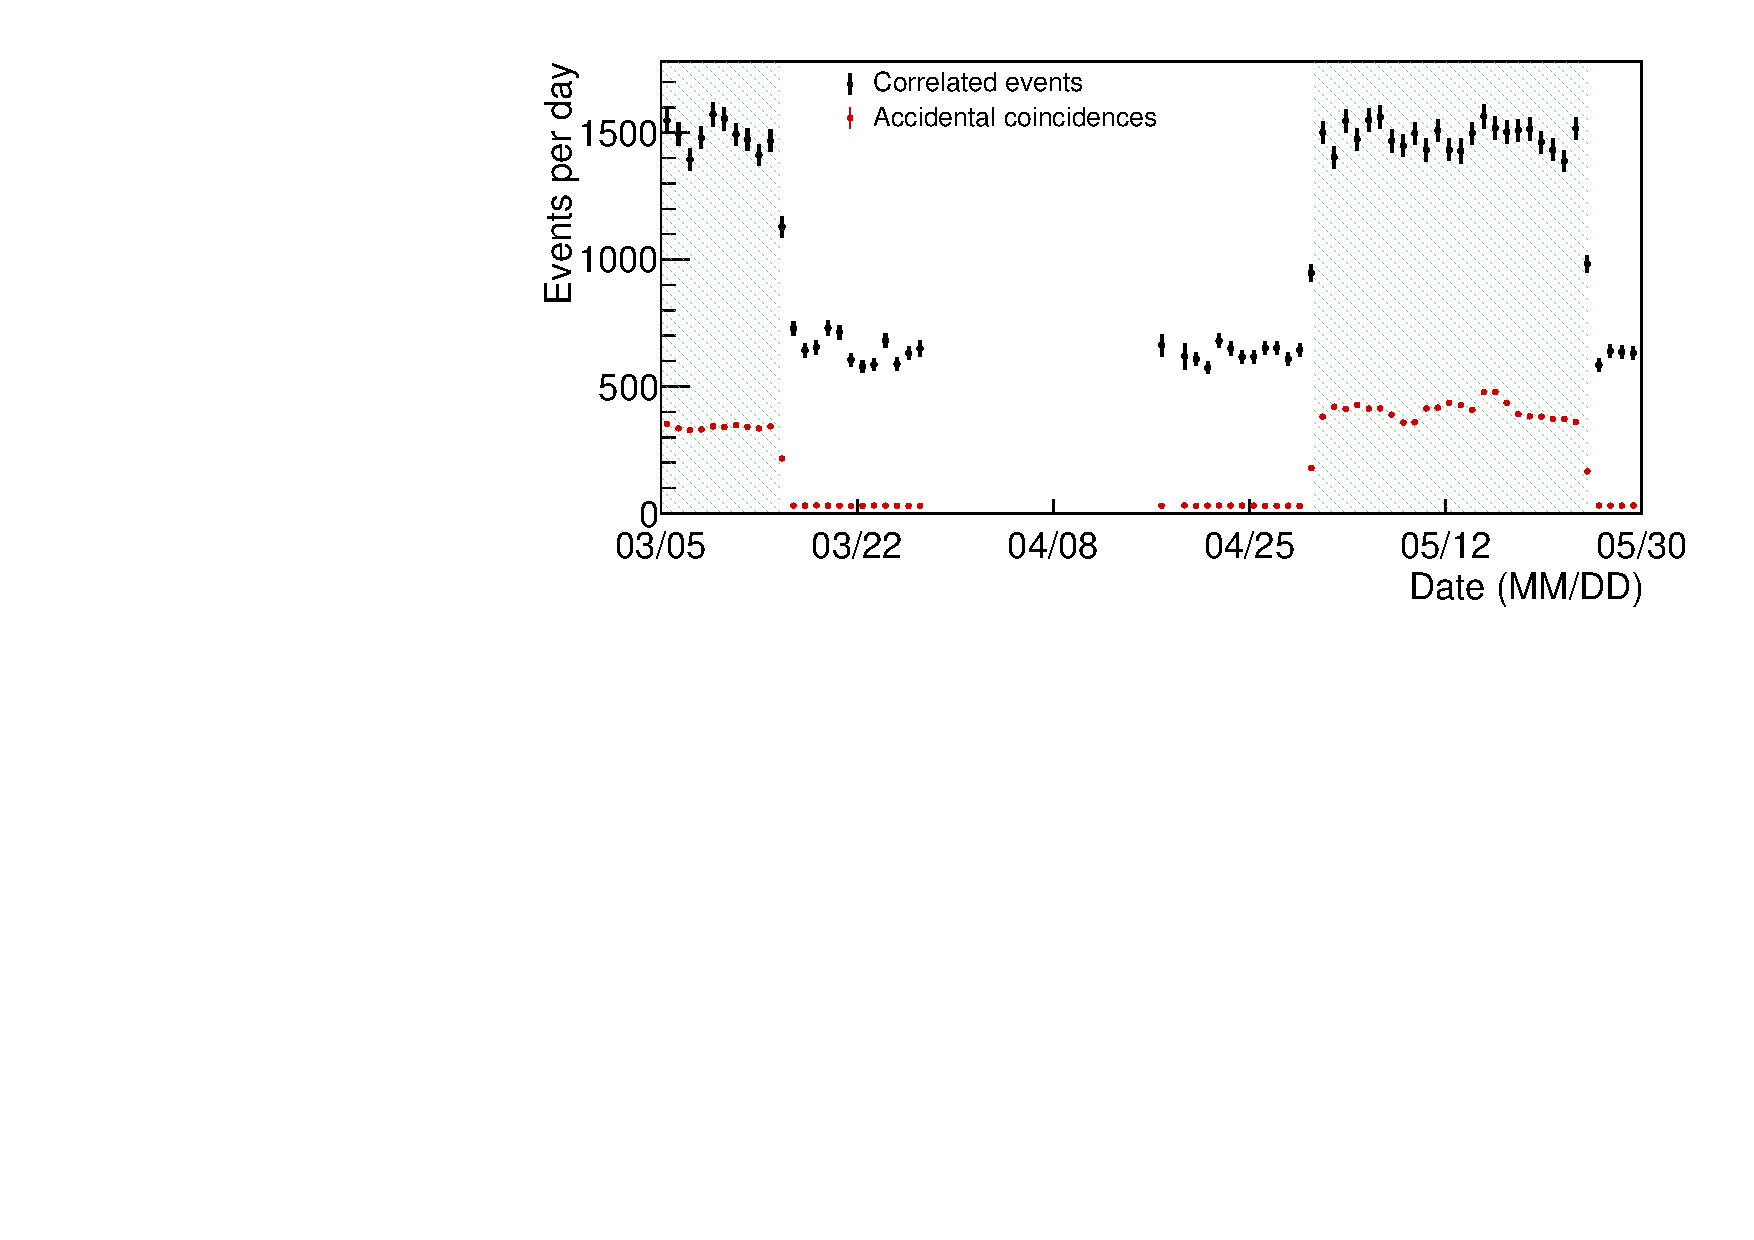
\includegraphics[width=0.9\linewidth]{tex/7-oscillation-images/EvtRates}
	\caption{Accidentals-subtracted IBD candidate event rate per day (black) and measured accidental rate (red) as a function of time. IBD candidate rates are corrected for dead time and exposure time. The shaded regions (green) are reactor on periods. Errors are statistical. The gap in data corresponds to a detector maintenance period.}
	\label{fig:evtrates}
\end{figure}


\section{IBD Rates versus Basline}

IBD rates as a function of distance from the reactor, $r$, are expected to fall as $1/r^2$. 
The fiducial volume of the reactor was divided into 14 baselines and the IBD rate at each baseline, scaled by active mass and relative efficiency, is plotted in Figure~\ref{fig:ibdvsbaseline}.
The data shows good agreement with a fit of the form $C/r^2$, producing a $\chi^2/NDF = 10.89/13$, confirming the inverse square law behavior. 
It can be noted that there is $\sim$40\% decrease in flux from the front to the back of the detector. 

\begin{figure}[H]
	\centering
	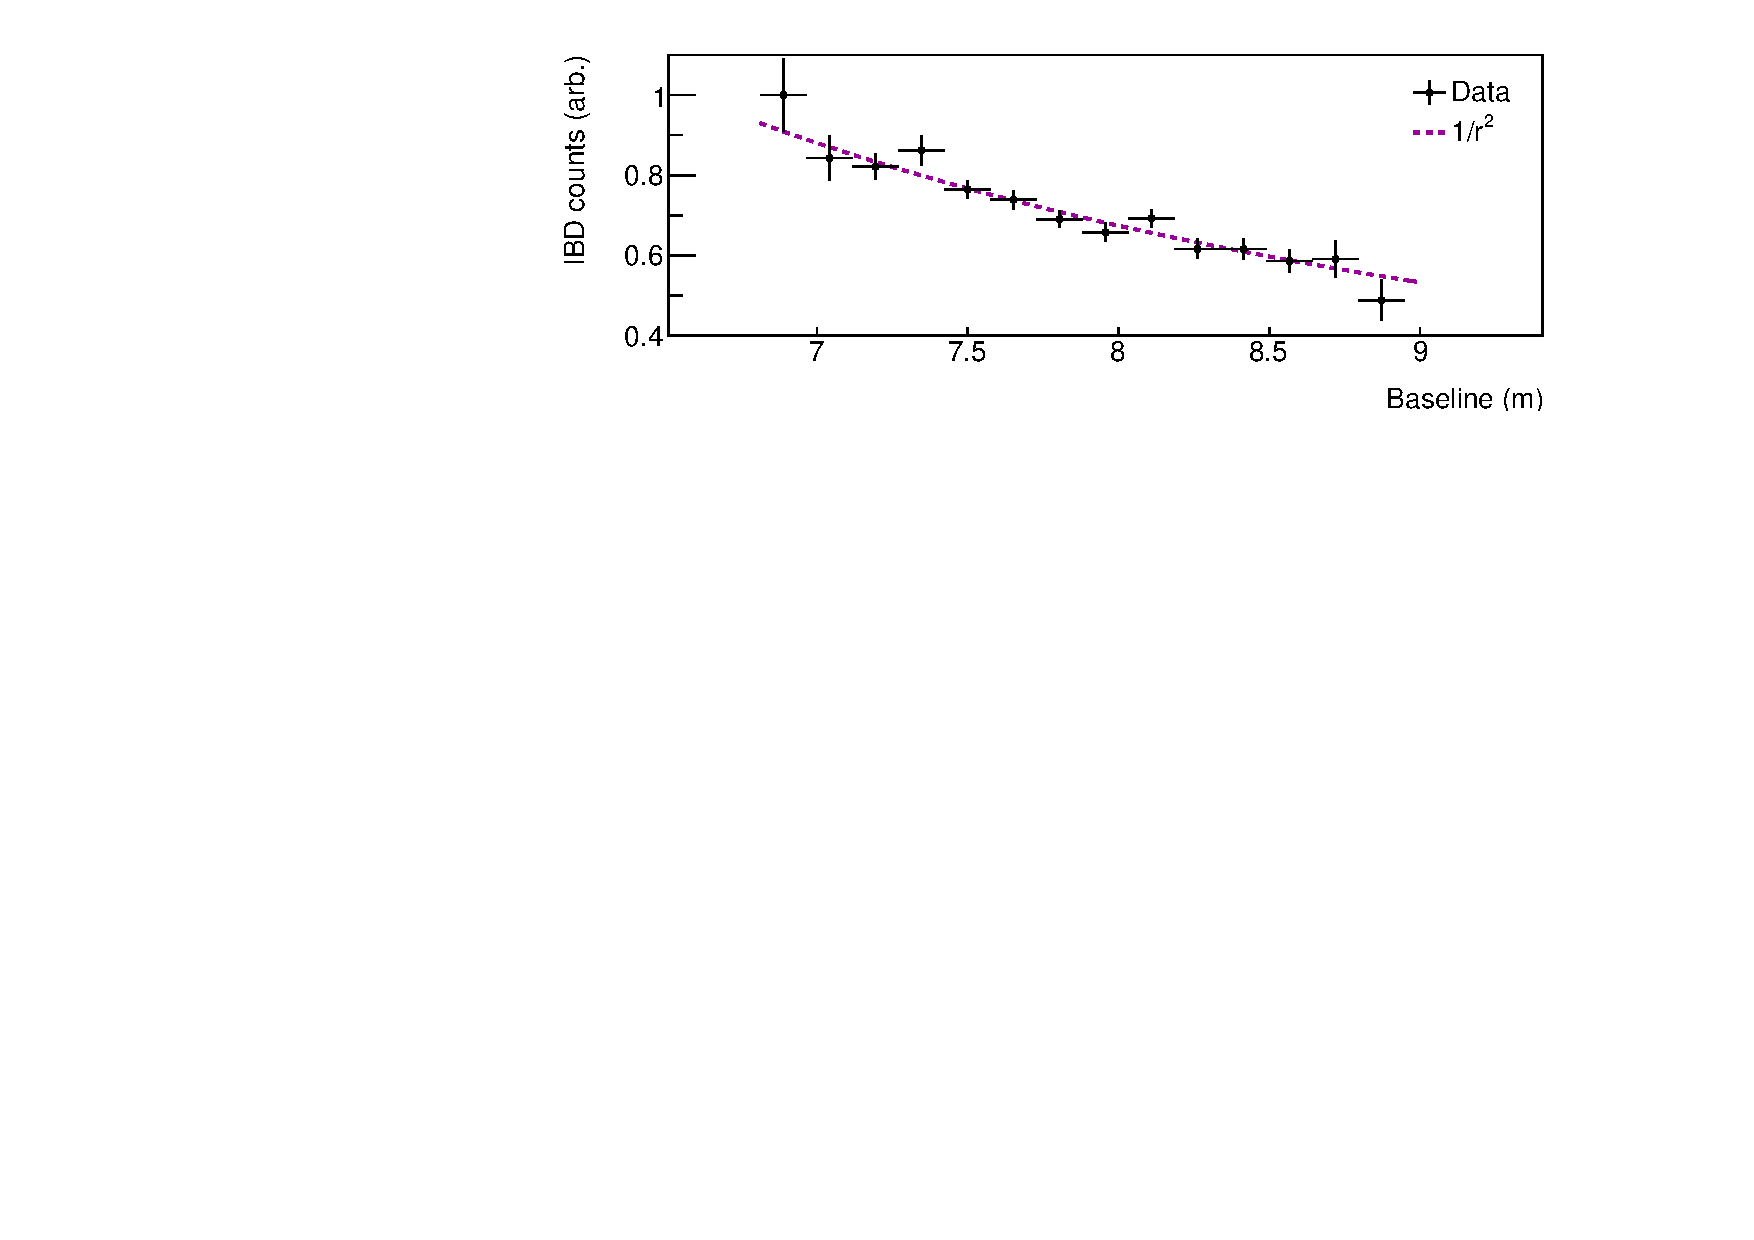
\includegraphics[width=1\linewidth]{tex/7-oscillation-images/IBDvsBaseline}
	\caption{Background subtracted IBD event rate as a function of distance from the reactor center binned into 14 unique baselines. Data is fit with $C/r^2$ (dashed, magenta) and produces a $\chi^2/NDF = 10.89/13$. Errors are statistical.}
	\label{fig:ibdvsbaseline}
\end{figure}

\todo{Correct for Ac-227 results and show corrected plot}


\section{Oscillation Search}

The construction of PROSPECT as a segmented detector allows the comparison of $\bar{\nu_e}$ spectrum between baselines rather than to a calculated reactor $\bar{\nu_e}$ spectrum. 
Therefore, the search for a sterile neutrino was carried out by comparing the measured IBD spectrum as a function of baseline (the L vs E spectrum) to a predicted L vs E spectrum constructed using MC simulations. 
The MC unoscillated prompt spectrum, $P_{null}(L,E_p)$, is described by:
\begin{equation}
	P_{null}(L,E_p) = W_{th} \cdot S(E_\nu)/4\pi L^2 \cdot t \cdot \epsilon_D(L,E_\nu,E_p) \cdot \rho_PV_D \cdot \sigma(E)
\end{equation}
where $W_{th}$ is the thermal power of the reactor, $S(E_\nu)$ is the $\bar{\nu_{e}}$ spectrum at energy E, $L$ is the given baseline, $t$ is the exposure time, $\rho_P$ is the proton density of the LS, $V_D$ is the active volume of the detector, $\sigma(E)$ is the IBD cross-section, and $\epsilon_D(L,E_\nu,E_p)$ is the detection efficiency and encompasses all detector effects.
This prompt spectrum is divided into 6 baseline (position) bins and 16 energy bins to create the L vs E spectra.

To compare the spectra at different baselines a covariance-matrix based $\chi^2$ test-statistic was built according to:
\begin{equation}	
	\chi^2 = \mathbf{\Delta^TV^{-1}_{tot}\Delta}
	\label{eq:chiosc}
\end{equation}
where $\mathbf{V_{tot}}$ is a covariance matrix constructed from the statistical and systematic uncertainties.
$\mathbf{\Delta}$ is a 96-element vector representing the relative agreement between the measured ($M_{l,e}$) and predicted ($P_{l,e}$) L vs E spectra in the $l^{th}$ baseline bin and $e^{th}$ energy bin:
\begin{equation}
	\Delta_{l,e} = M_{l,e} - M_e\frac{P_{l,e}}{P_e}.
	\label{eq:deltaosc}
\end{equation}
$M_e$ and $P_e$ are the detector-wide spectrum rates in the $e^{th}$ energy bin and are defined as
\begin{equation}
	M_e = \sum_{l=1}^{6}M_{l,e}~\textrm{and}~P_e = \sum_{l=1}^{6}P_{l,e}.
\end{equation}

The predicted L vs E spectrum is modeled to include sterile neutrino oscillations as
\begin{equation}
	P_{l,e}(\Delta m_{14}^2,\theta_{14}) = P_{l,e}(0,0)\left(1-sin^22\theta_{14}sin^2\left(1.27\Delta m_{14}^2\frac{L}{E}   \right)\right)
\end{equation}
where $m_{14}^2$ and $\theta_{14}$ describe mixing between one active neutrino flavor state and one sterile neutrino state.
The search for sterile neutrino oscillations is then carried out by minimizing the $\chi^2$ in Equation~\ref{eq:chiosc} by varying the parameters $m_{14}^2$ and $\theta_{14}$.

\subsection{Uncertainties}

Statistical and systematic uncertainties are included in the form of covariance matrices $\mathbf{V_{stat}}$ and $\mathbf{V_{syst}}$.
The statistical uncertainties are directly calculated from data using Poisson statistics, resulting in an uncorrelated, diagonal matrix.
Since the predicted L vs E spectra are normalized by the baseline-integrated spectra rates ($M_e$), as shown in Equation~\ref{eq:deltaosc}, off-diagonal terms need to be added to take into account the correlation between $M_{l,e}$ and $M_e$.
Therefore, the full statistical covariance matrix is included as:
\begin{equation}
	V_{stat,l,e} = \sigma^2_{stat,l,e}\left(1-2\frac{M_{l,e}}{M_e}\right) + \sigma^2_{stat,e}\left(\frac{M_{l,e}}{M_e}\right)^2
\end{equation}
Beyond this, additional off-diagonal terms are included to account for correlations between position bins with the same energy arising from the use of $M_e$.
These corrections were estimated by studying Monte Carlo toy's and extracting the resulting covariance matrix.

For each systematic uncertainty a normalized covariance matrix is produced using toy MC datasets and varying each systematic by 1$\sigma$.
Assuming that all errors are Gaussian, the total covariance matrix is then calculated as the sum of all statistical and systematic matrices as
\begin{equation}
	\mathbf{V_{tot}} = \mathbf{V_{stat}} + \sum_{i}\mathbf{V_{syst,i}}.
\end{equation}

In addition to uncertainties from statistics and detector response, uncertainties about the reactor $\bar{\nu_{e}}$ flux have to be taken into account.
The MC $\bar{\nu_{e}}$ spectrum is generated using the Huber $^{235}$U flux model \cite{Huber} and the Vogel-Beacom model for IBD cross section \cite{Vogel:1999zy}, not taking into account $\bar{\nu_{e}}$'s that may be generated via processes other than by $^{235}$U fission.
The fuel used in the HFIR reactor core is U$_3$O$_8$-Al, allowing the possibility of $\bar{\nu_{e}}$ production through neutron activation of the $^{27}$Al:
\begin{equation}
	^{27}_{13}Al + ^1_0n \rightarrow ^{28}_{14}Al \rightarrow ^{28}_{14}Si + \beta^- + \bar{\nu_{e}}
\end{equation}
$^{28}$Al has a half-life of 2.245 minutes with an endpoint energy of 2.86 MeV \cite{ENSDF}, producing low energy $\bar{\nu_{e}}$'s.
This process was modeled \cite{ConantThesis}, and aluminum corrections were estimated to contribute $\sim$0.85\% over the full dataset, all with energies below 3 MeV as seen in Figure~\ref{fig:alcontrib} \cite{PSurukuchi:2338}. 

Furthermore, a correction is needed for $\bar{\nu_{e}}$'s produced by long-lived fission isotopes (non-equilibrium isotopes).
The ILL beta-spectrum measurements \cite{VonFeilitzsch:1982jw, Schreckenbach:1985ep, Hahn:1989zr}, which are used in the Huber spectrum, are based on $\sim$1-day long measurements, compared to an average HFIR reactor cycle, which is about 24 days.
As there are a number of long-lived isotopes, their $\bar{\nu_{e}}$ contributions were not included in the Huber model but do contribute the spectrum measured by PROSPECT.
Extrapolating from predictions made in~\cite{Mueller}, non-equilibrium corrections were found to be $\sim$0.5\% over the full dataset, with most contributions below 4 MeV as seen in Figure~\ref{fig:noneqcontrib} \cite{PSurukuchi:2346}.

Including both the aluminum and non-equilibrium contributions to the $\bar{\nu_{e}}$ spectrum results in a 1.3\% increase in the model spectrum, shown in Figure~\ref{fig:spectrumwithcorrections}.
For a summary of all systematic uncertainties see Table~\ref{tab:sysunc}.

\begin{figure}[H]
	\centering
	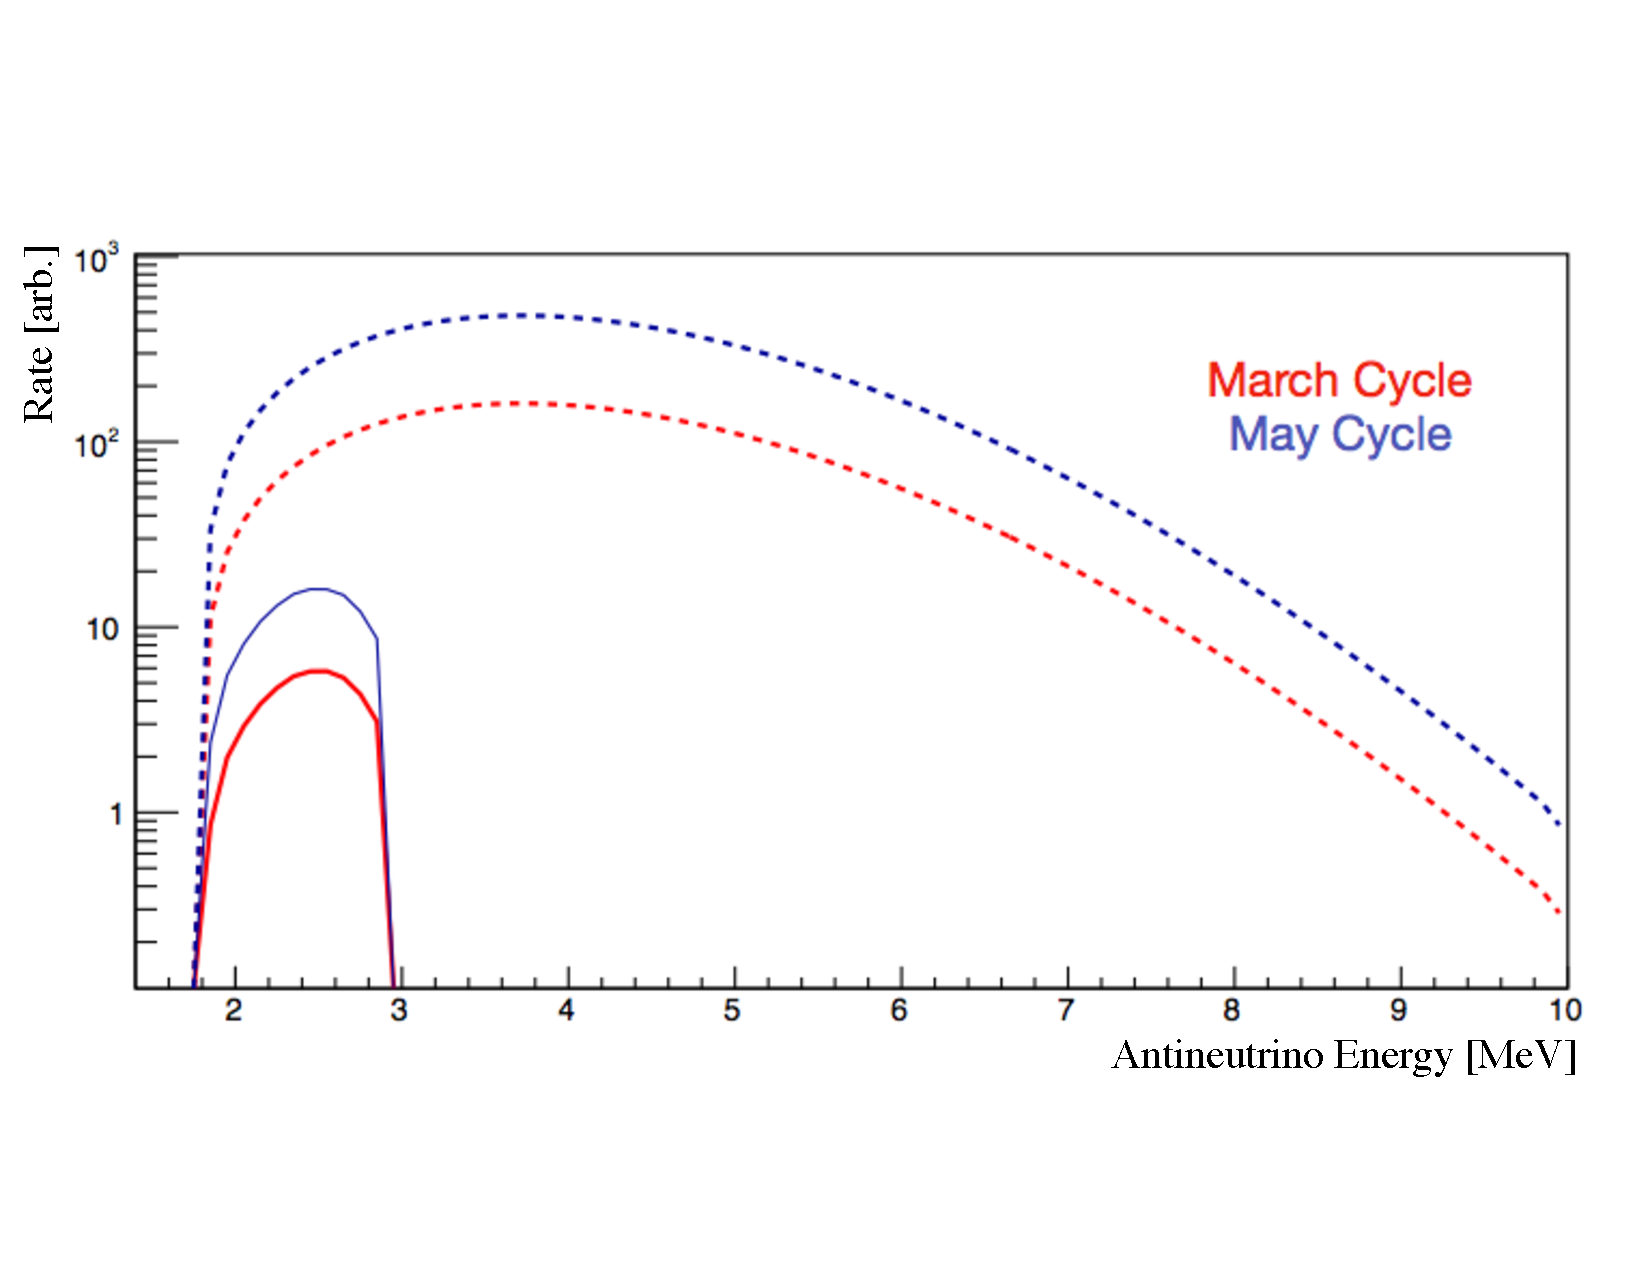
\includegraphics[width=0.6\linewidth]{tex/7-oscillation-images/AlContrib}
	\caption[]{$\bar{\nu_{e}}$ spectrum from $^{28}$Al $\beta$-decay (solid) and $^{235}$U fission (dashed) for both reactor on cycles used in this analysis \cite{PSurukuchi:2338}}.
	\label{fig:alcontrib}
\end{figure}

\begin{figure}[H]
	\centering
	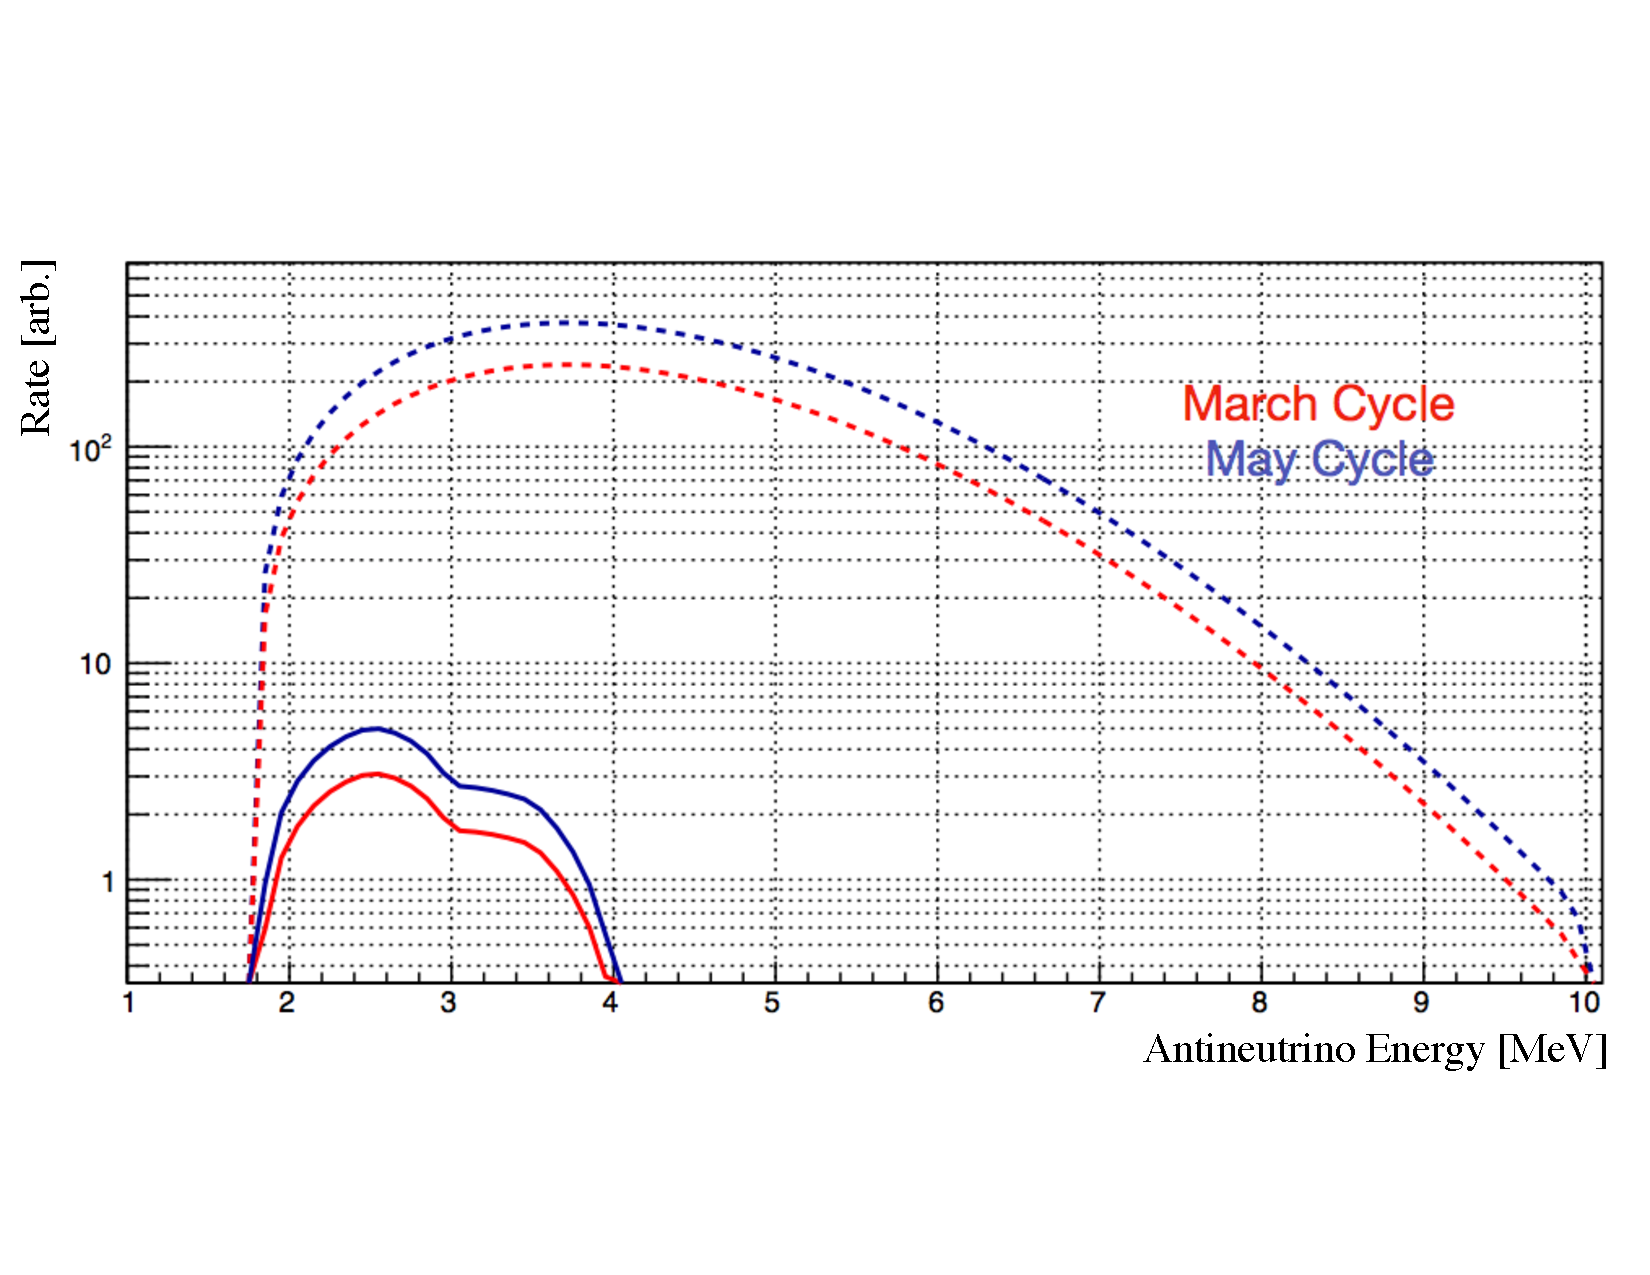
\includegraphics[width=0.6\linewidth]{tex/7-oscillation-images/NonEqContrib}
	\caption[]{$\bar{\nu_{e}}$ spectrum from non-equilibrium isotopes (solid) and $^{235}$U fission (dashed) for both reactor on cycles uses in this analysis \cite{PSurukuchi:2346}.}
	\label{fig:noneqcontrib}
\end{figure}

\begin{figure}[H]
	\centering
	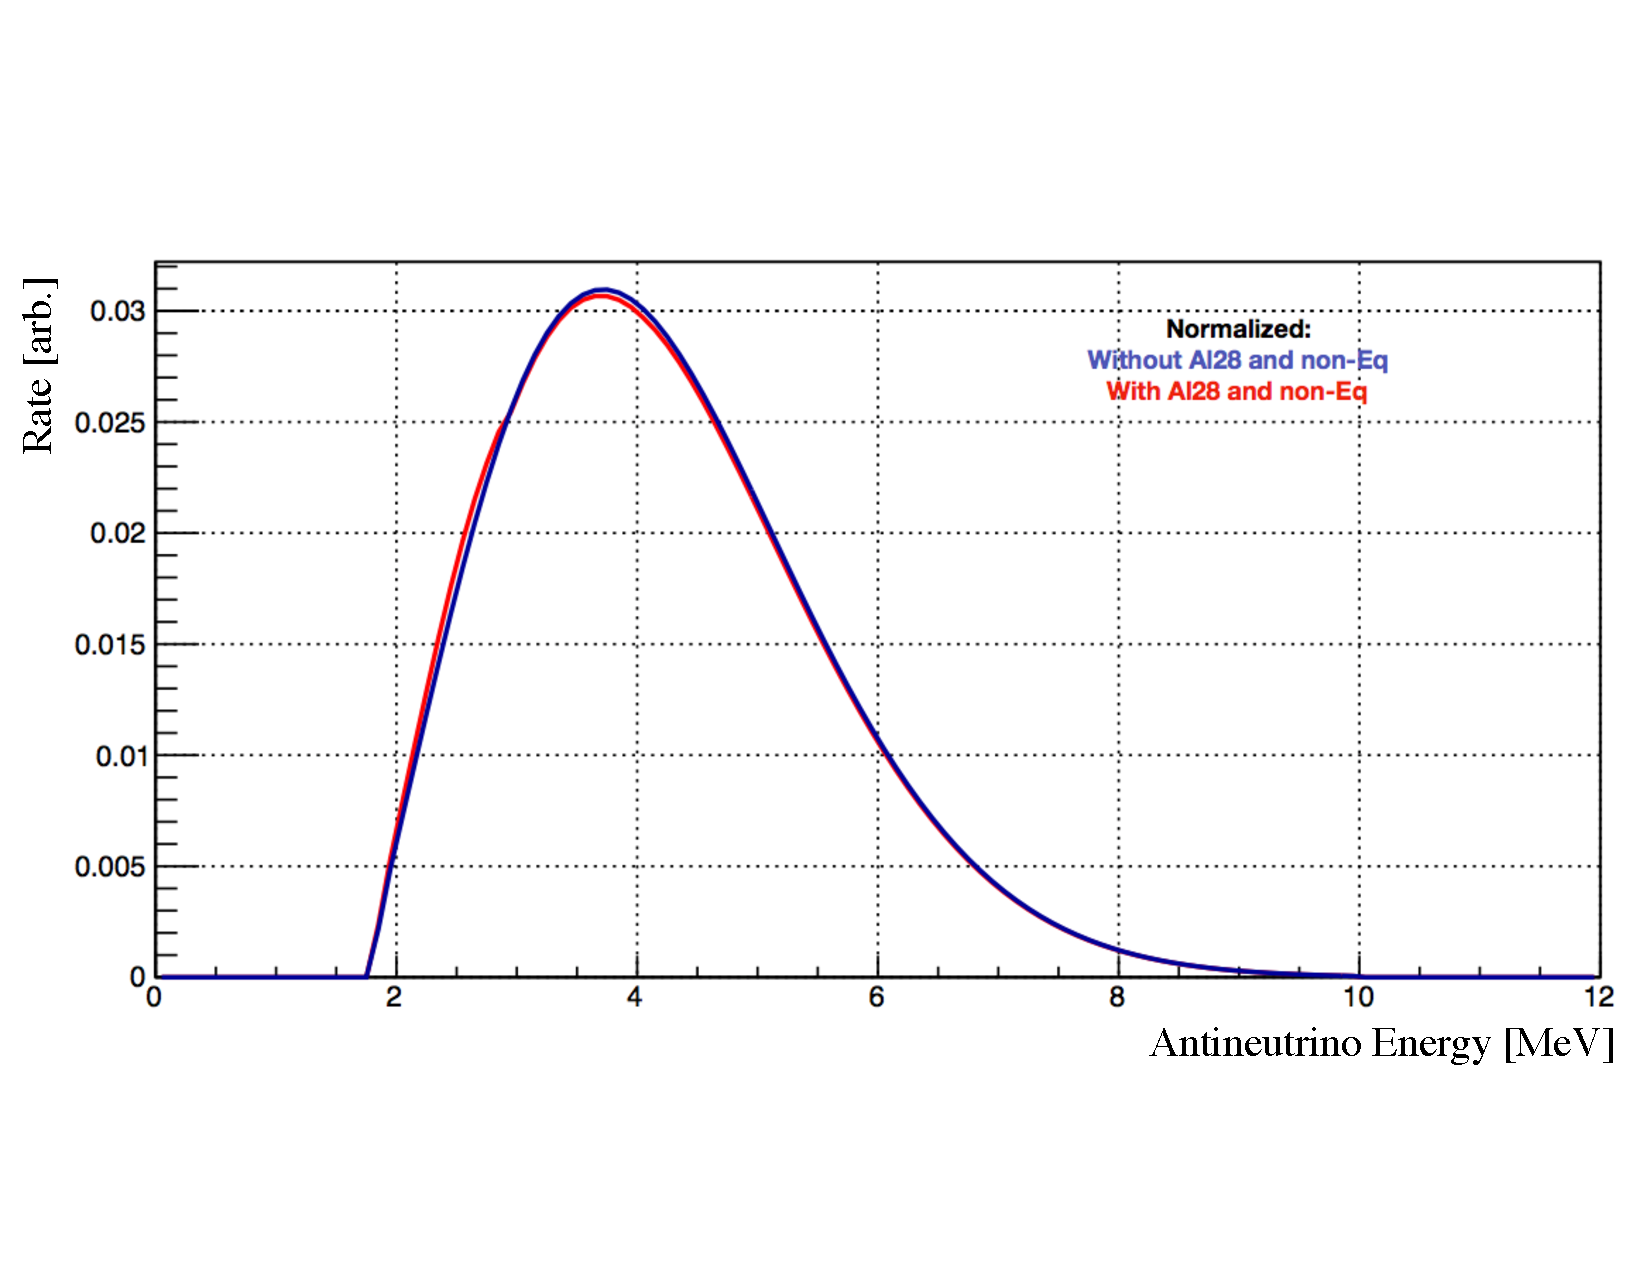
\includegraphics[width=0.7\linewidth]{tex/7-oscillation-images/SpectrumWithCorrections}
	\caption{The normalized $\bar{\nu_{e}}$ as predicted by Huber+Vogel-Beacom with and without the aluminum + non-equilibrium corrections (1.3\%).}
	\label{fig:spectrumwithcorrections}
\end{figure}

\begin{table}[H]
\centering
\begin{tabular}{lcc}
	\hline 
	\textbf{Parameter} & \textbf{Nominal Value} & \textbf{Uncertainty} \\ 
	\hline 
	Background normalization  & - & 5\% \\ 
	Uncorrelated (n,H) to (n,C$^*$) peak & - & 5\% \\ 
	Background scaling & - & 0.2\% \\ 
	\hline 
	Birks' nonlinearity ($k_{B1}$) & 0.100 mm/MeV & 0.012 mm/MeV \\ 
	Cherenkov nonlinearity ($k_c$) & 51\% & 4\% \\ 
	Energy scale ($A$) & 1 & 0.7\% \\ 
	Energy resolution & 4.45\% & 0.2\% \\ 
	Energy loss & - & 30 keV \\ 
	Uncorrelated IBD efficiency & - & 5\% \\ 
	Uncorrelated volume & - & per segment \\ 
	Uncorrelated energy resolution & 4.45\% & 0.2\% \\ 
	Uncorrelated energy loss  & - & 30 keV \\ 
	Baseline uncertainty & 793.2 cm & 10 cm \\ 
	\hline 
	$^{28}$Al spectrum correction & - & 100\% \\ 
	Non-equilibrium spectrum correction & - & 100\% \\ 
	\hline 
\end{tabular} 
\caption{Summary of systematic uncertainties that were used to generate the covariance matrices used in the oscillation analysis. Uncertainties are correlated unless otherwise noted.}
\label{tab:sysunc}
\end{table}

\subsection{Confidence Interval Assignment}

The frequentist approach proposed by Feldman and Cousins \cite{PhysRevD.57.3873} was used to assign confidence intervals for the oscillation analysis.
This was done by defining a critical $\Delta\chi^2_C$ value for each point on the $\sin^22\theta_{14}-\Delta m^2_{14}$ grid for a chosen confidence level.

For each point on the $\sin^22\theta_{14}-\Delta m^2_{14}$ grid 1000 oscillated MC toy datasets are generated, fluctuating the statistical and systematic uncertainties.
For each of these toys a minimum $\chi^2_{min}$ is found by applying Equation~\ref{eq:chiosc}.
Then, a $\Delta\chi^2$ is defined as
\begin{equation}
	\Delta\chi^2 = \chi^2_{min,true} - \chi^2_{min,best-fit}
\end{equation}
where $\chi^2_{min,true}$ and $\chi^2_{min,best-fit}$ are the $\chi^2_{min}$ for the true oscillation parameters and best-fit parameters for that given toy.

Then, for each point on the grid a $\Delta\chi^2_C$ was defined for a given confidence level $\alpha$ such that
\begin{equation}
	\frac{\sum_{0}^{\Delta\chi^2_C}P(\Delta\chi^2)}{\sum_{0}^{\infty}P(\Delta\chi^2)} = \alpha
\end{equation}
where $P(\Delta\chi^2)$ is the distribution of $\Delta\chi^2$ for all toys for the given grid point.
See Figure~\ref{fig:chi2map} for the distribution of $\Delta\chi^2_C$ values for $\alpha = 95\%$.
A point on the $\sin^22\theta_{14}-\Delta m^2_{14}$ grid is said to be excluded by data at a $\alpha$ confidence level if $\Delta\chi^2_{data} > \Delta\chi^2_{C}$ where $\Delta\chi^2_{data}$ is the difference between the data and best-fit minimized $\chi^2$.


\begin{figure}[h]
	\centering
	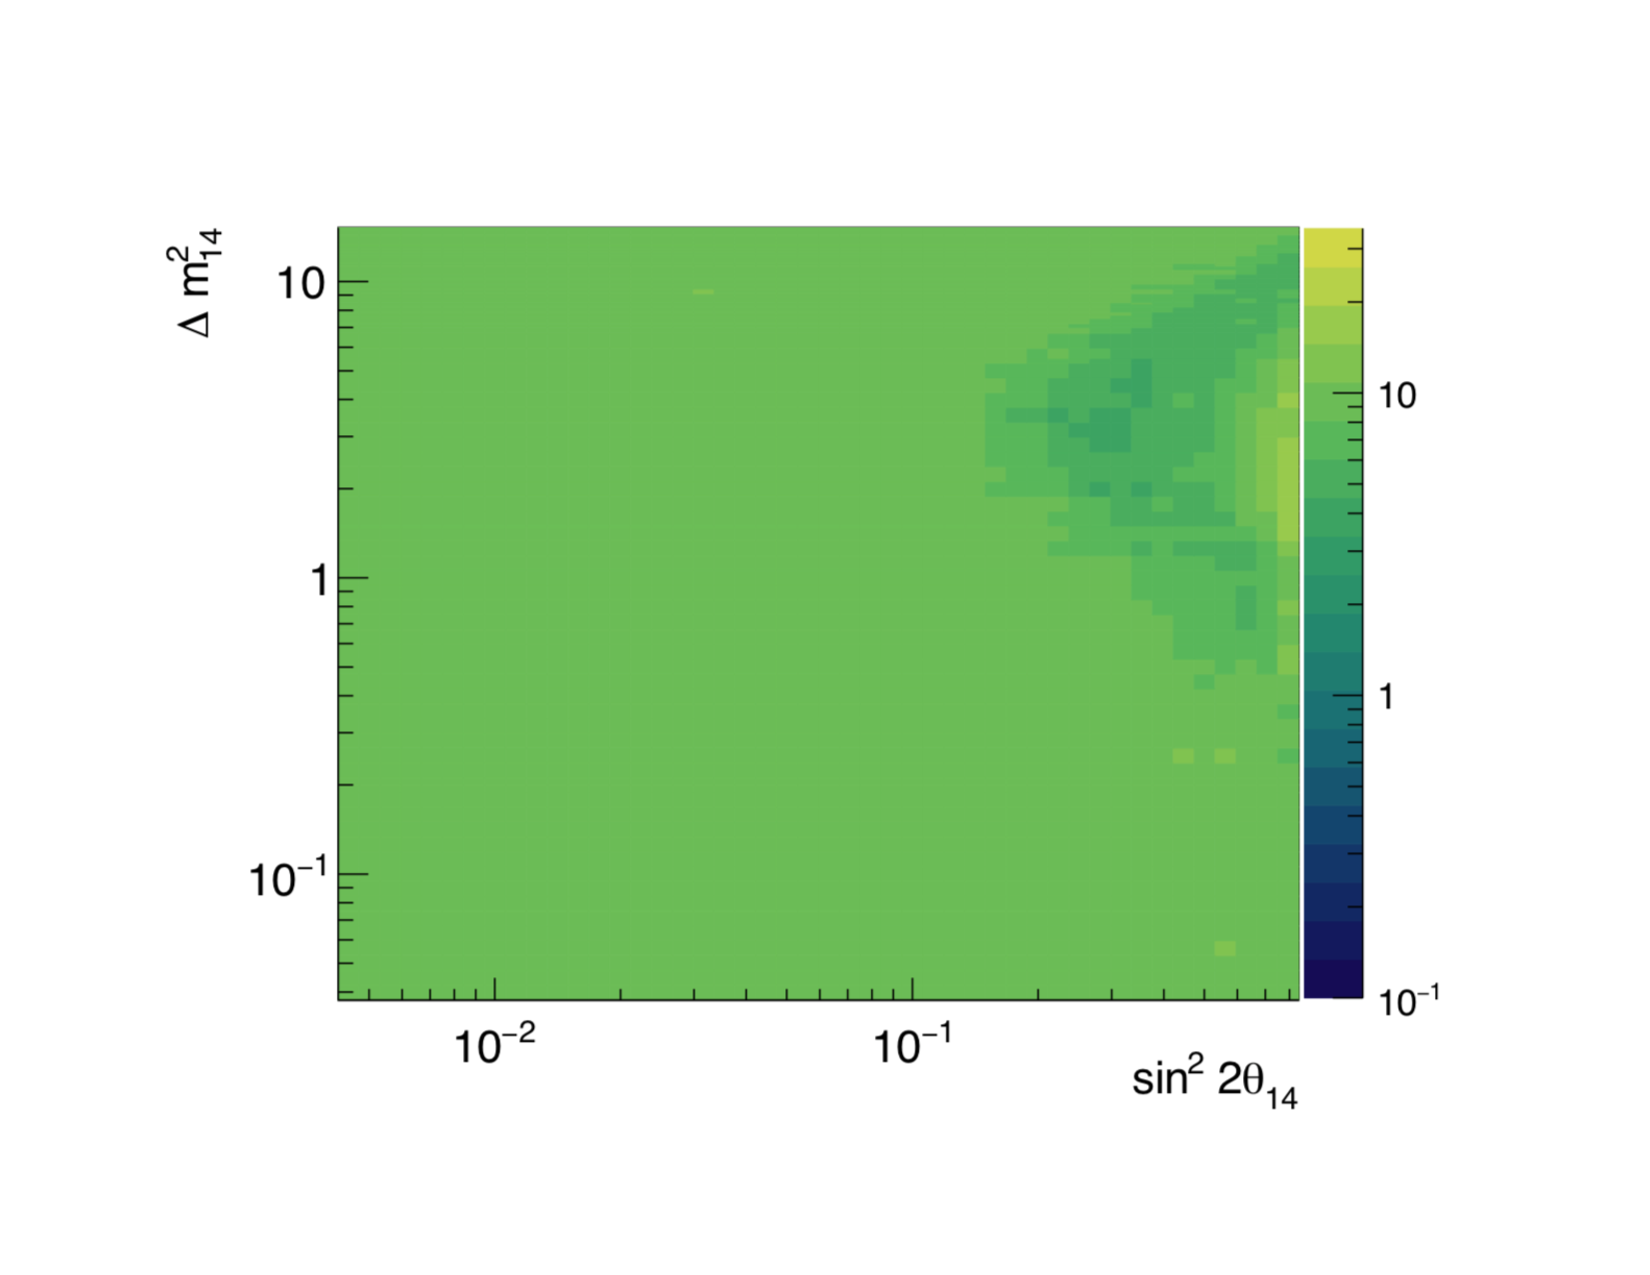
\includegraphics[width=0.7\linewidth]{tex/7-oscillation-images/Chi2Map}
	\caption[]{Critical $\Delta\chi^2_C$ values for a 95\% confidence level \cite{SurukuchiThesis}.}
	\label{fig:chi2map}
\end{figure}


\subsection{Results}

For each baseline bin the ratio between the measured IBD prompt spectrum ($M_{l,e}$) to the total spectrum, normalized by the no-oscillation prediction (null hypothesis), ($M_e\frac{P_{l,e}}{P_e}$) for data, no-oscillation prediction, and the best-fit Reactor Antineutrino Anomaly oscillation parameters is shown in Figure~\ref{fig:baselinespectra}.
No significant deviations from the no-oscillation prediction are observed throughout the energy spectra at all chosen baselines.

The level of agreement between data and the null hypothesis can be quantified using the $\chi^2$ in Equation~\ref{eq:chiosc}.
At $\theta_{14} = 0$, the $\chi^2/NDF = 61.9/80$, indicating good agreement between the data and null hypothesis.
Allowing oscillations, a global minimum is found at $\Delta m^2_{41} = 0.5 \textrm{eV}^2$ and $\sin^22\theta_{14} = 0.35$, with $\chi^2/NDF = 57.9/78$.
A $p$ value for these results is generated by comparing the data $\Delta\chi^2$ values to the $\Delta\chi^2_C$ distributions. 
Comparison of the null and sterile neutrino hypotheses results in a $p$-value of 0.58, demonstrating that the PROSPECT data is compatible with the standard 3-flavor neutrino mixing framework.

Figure~\ref{fig:exclusionsensitivityfinal} shows the 95\% confidence level exclusion contour and expected sensitivity from the 33 days of reactor-on PROSPECT data.
The data-set used in this analysis excludes large portions of the Reactor Antineutrino Anomaly (RAA) allowed region and disfavors the RAA best-fit point at 2$\sigma$ confidence level with a $p$-value of 0.013.


\begin{figure}[H]
	\centering
	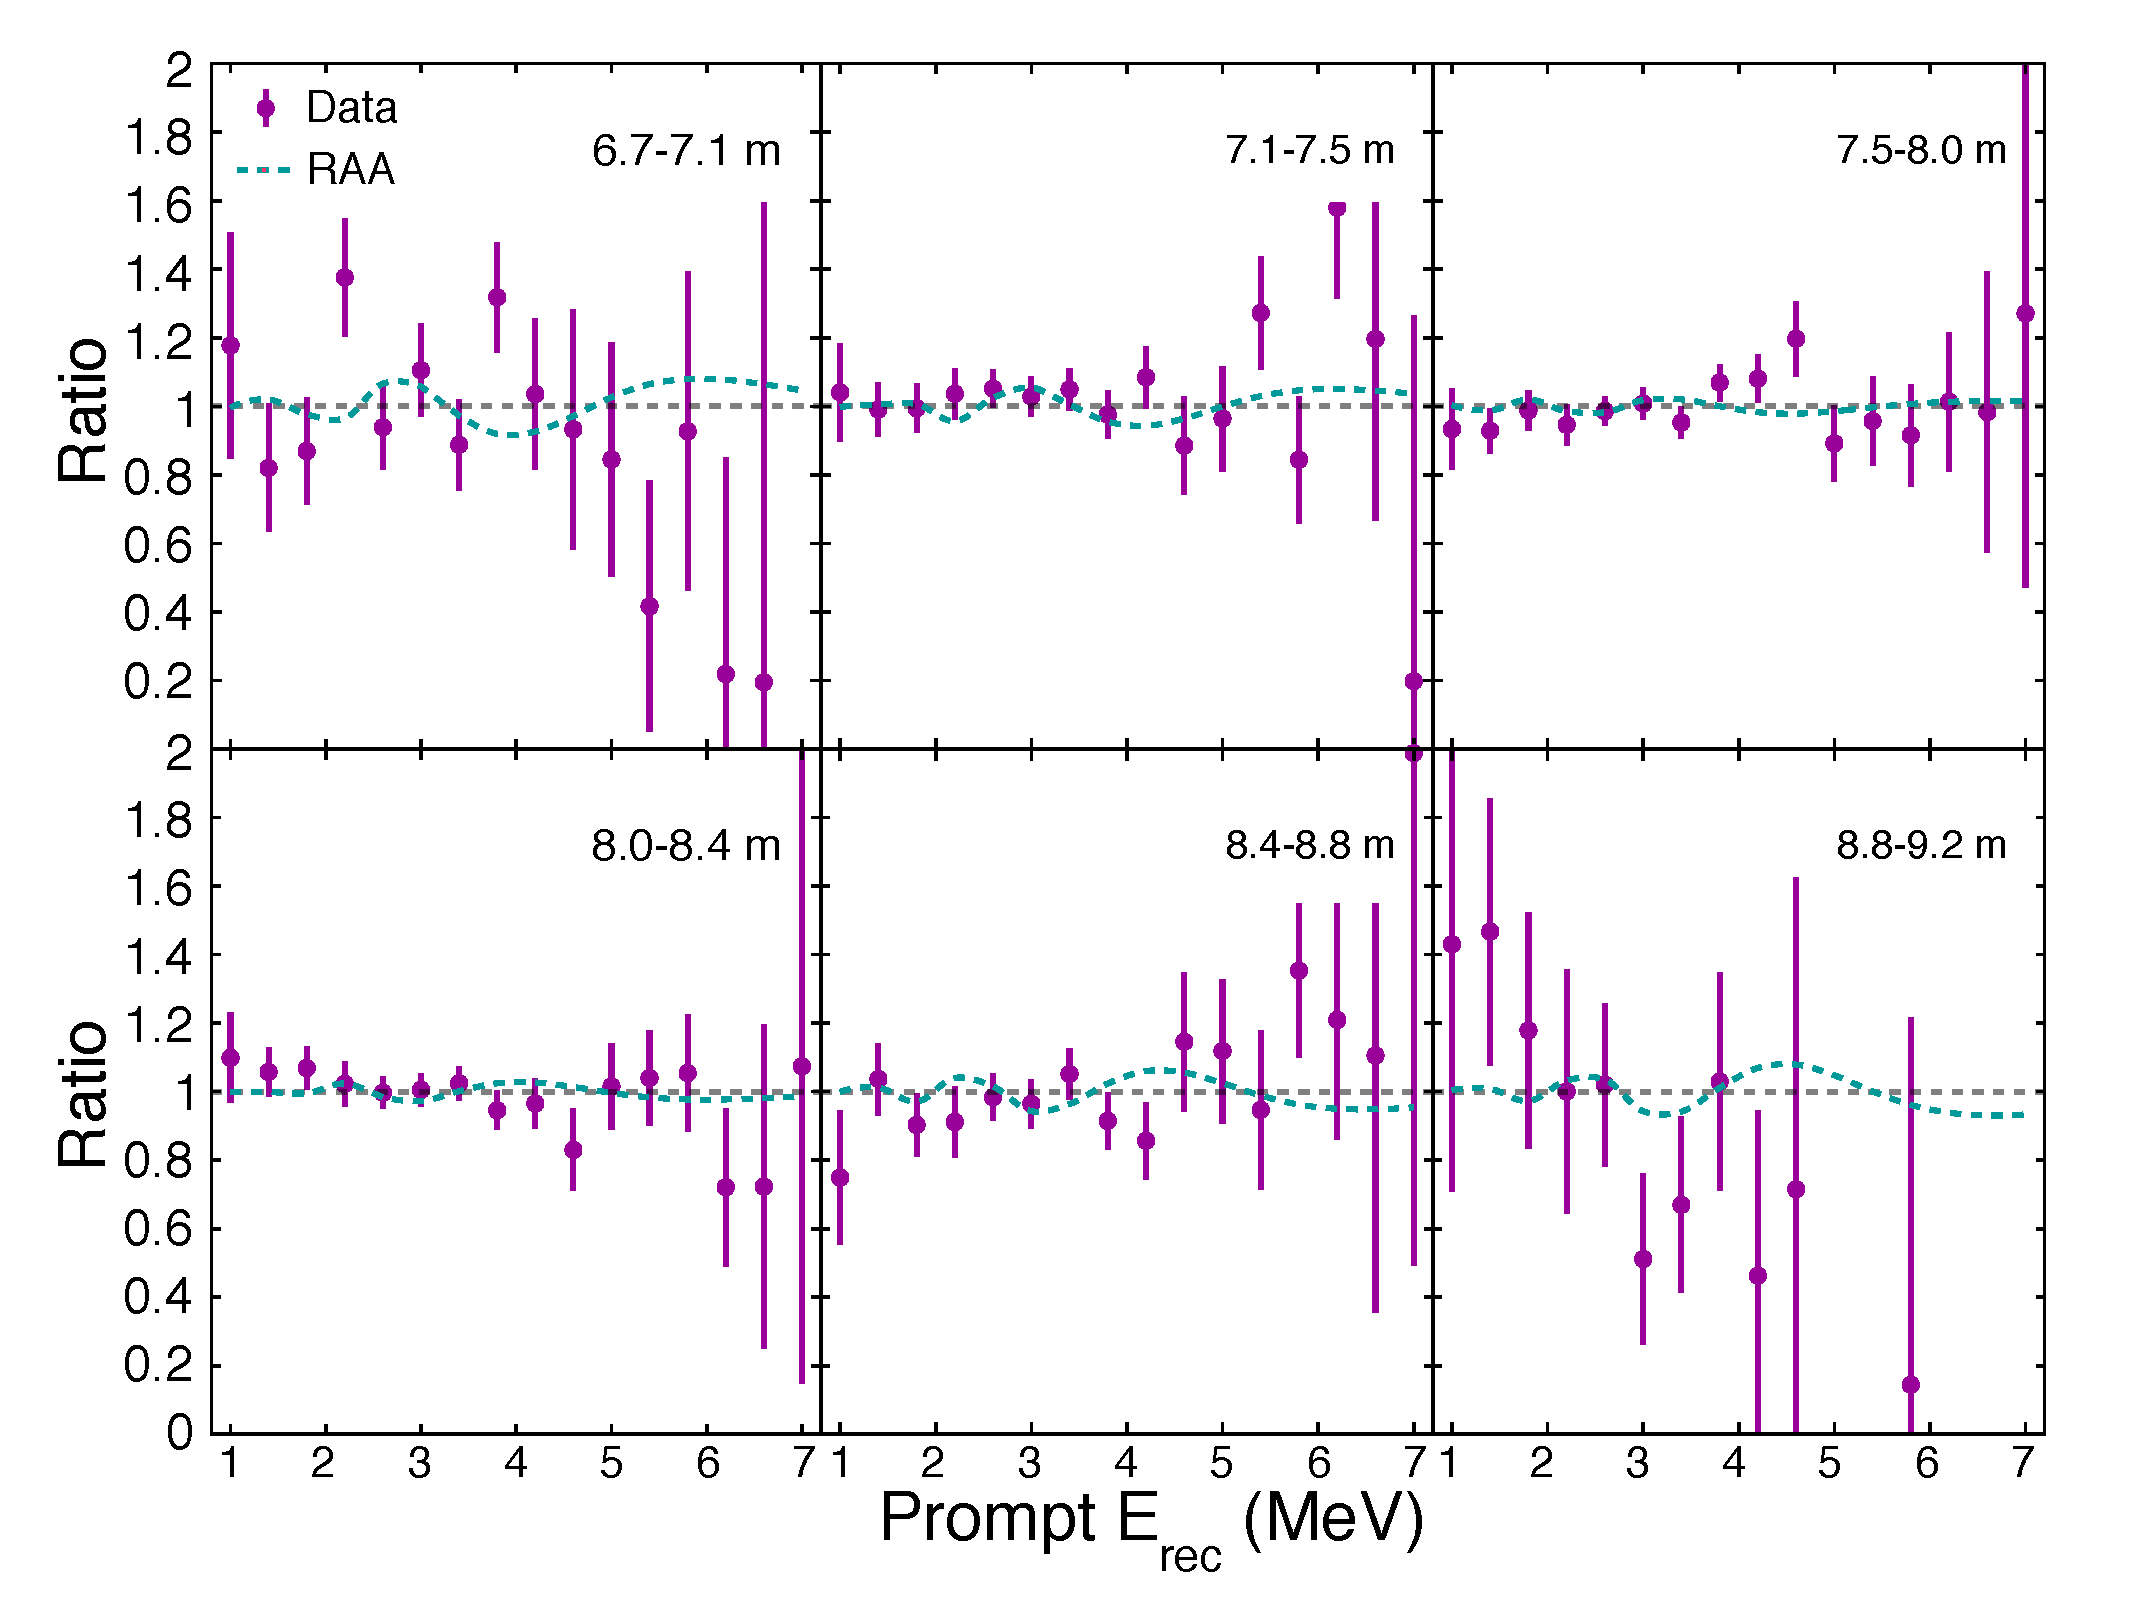
\includegraphics[width=0.9\linewidth]{tex/7-oscillation-images/BaselineSpectra}
	\caption{Ratio of the measured IBD prompt energy spectra to the predicted baseline-integrated spectrum, for 6 baseline bins. Error bars include statistical and systematic uncertainties. Also shown are the no-oscillation expectation (gray, dashed) and an oscillated expectation based on the best fit Reactor Antineutrino Anomaly parameters (teal, dashed). \cite{PhysRevLett.121.251802}}
	\label{fig:baselinespectra}
\end{figure}

\begin{figure}[H]
	\centering
	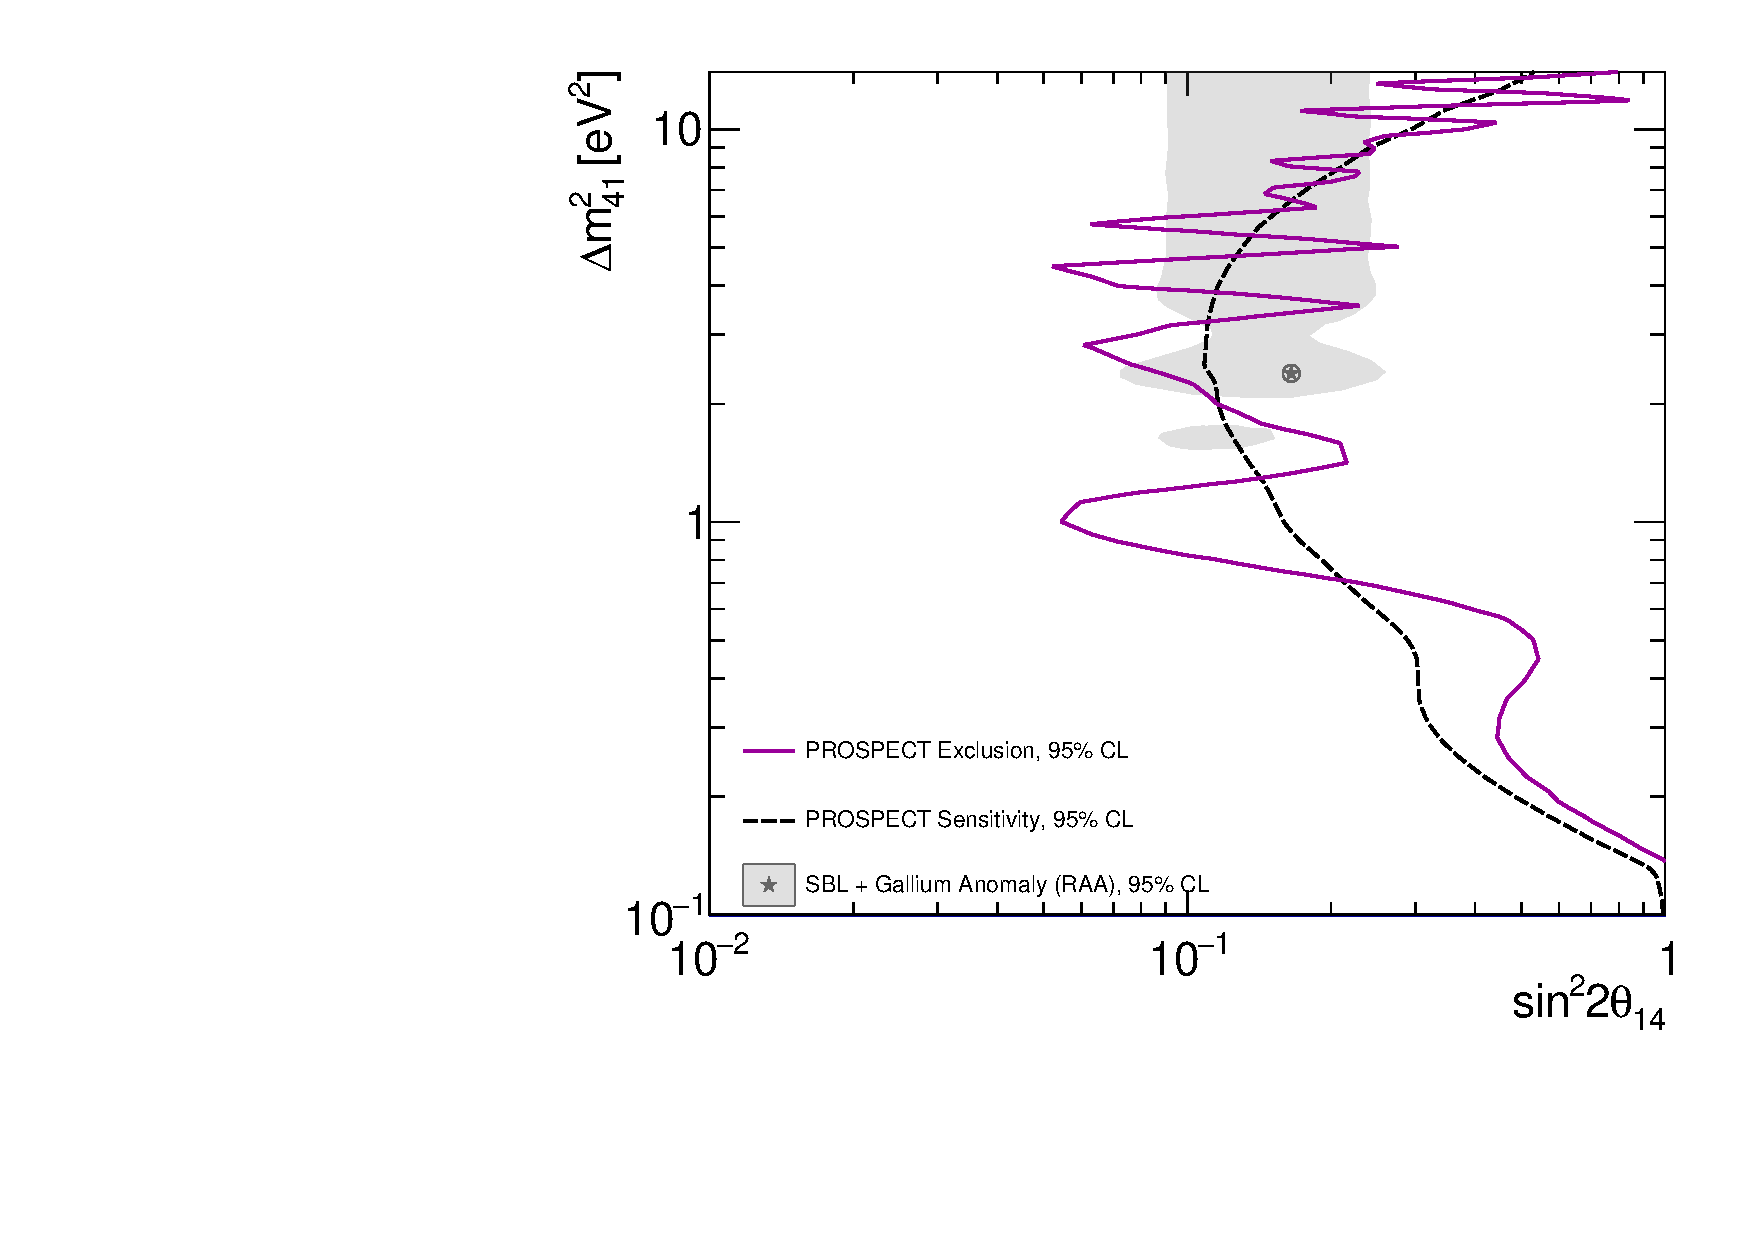
\includegraphics[width=0.7\linewidth]{tex/7-oscillation-images/Exclusion_Sensitivity_Final}
	\caption[]{Sensitivity and 95\% confidence level sterile neutrino oscillation exclusion contour from the 33 day reactor-on PROSPECT data set. The best fit parameters of the Reactor Antineutrino Anomaly (star) is disfavored at 2.2$\sigma$ confidence level. \cite{PhysRevLett.121.251802}}
	\label{fig:exclusionsensitivityfinal}
\end{figure}


\section{Measured Antineutrino Spectrum}

Selection criteria for IBD events used in the measurement the antineutrino spectrum were the same as those used in the oscillation analysis, with the exception of the shower veto.
The veto window around a cosmic muon cluster was increased to (0,200) $\mu$s, and around a fast neutron to (-250,+250) $\mu$s.
The analysis method for determining the prompt spectrum was also the same used for the oscillation analysis, a subtraction of accidental events from correlated events in both reactor on and off data sets.
An atmospheric correction factor of $k_p = 0.991 \pm 0.004$ was applied. 
The resulting prompt energy spectrum of IBD events can be seen in Figure~\ref{fig:spectrumresults}.


\begin{figure}[H]
	\centering
	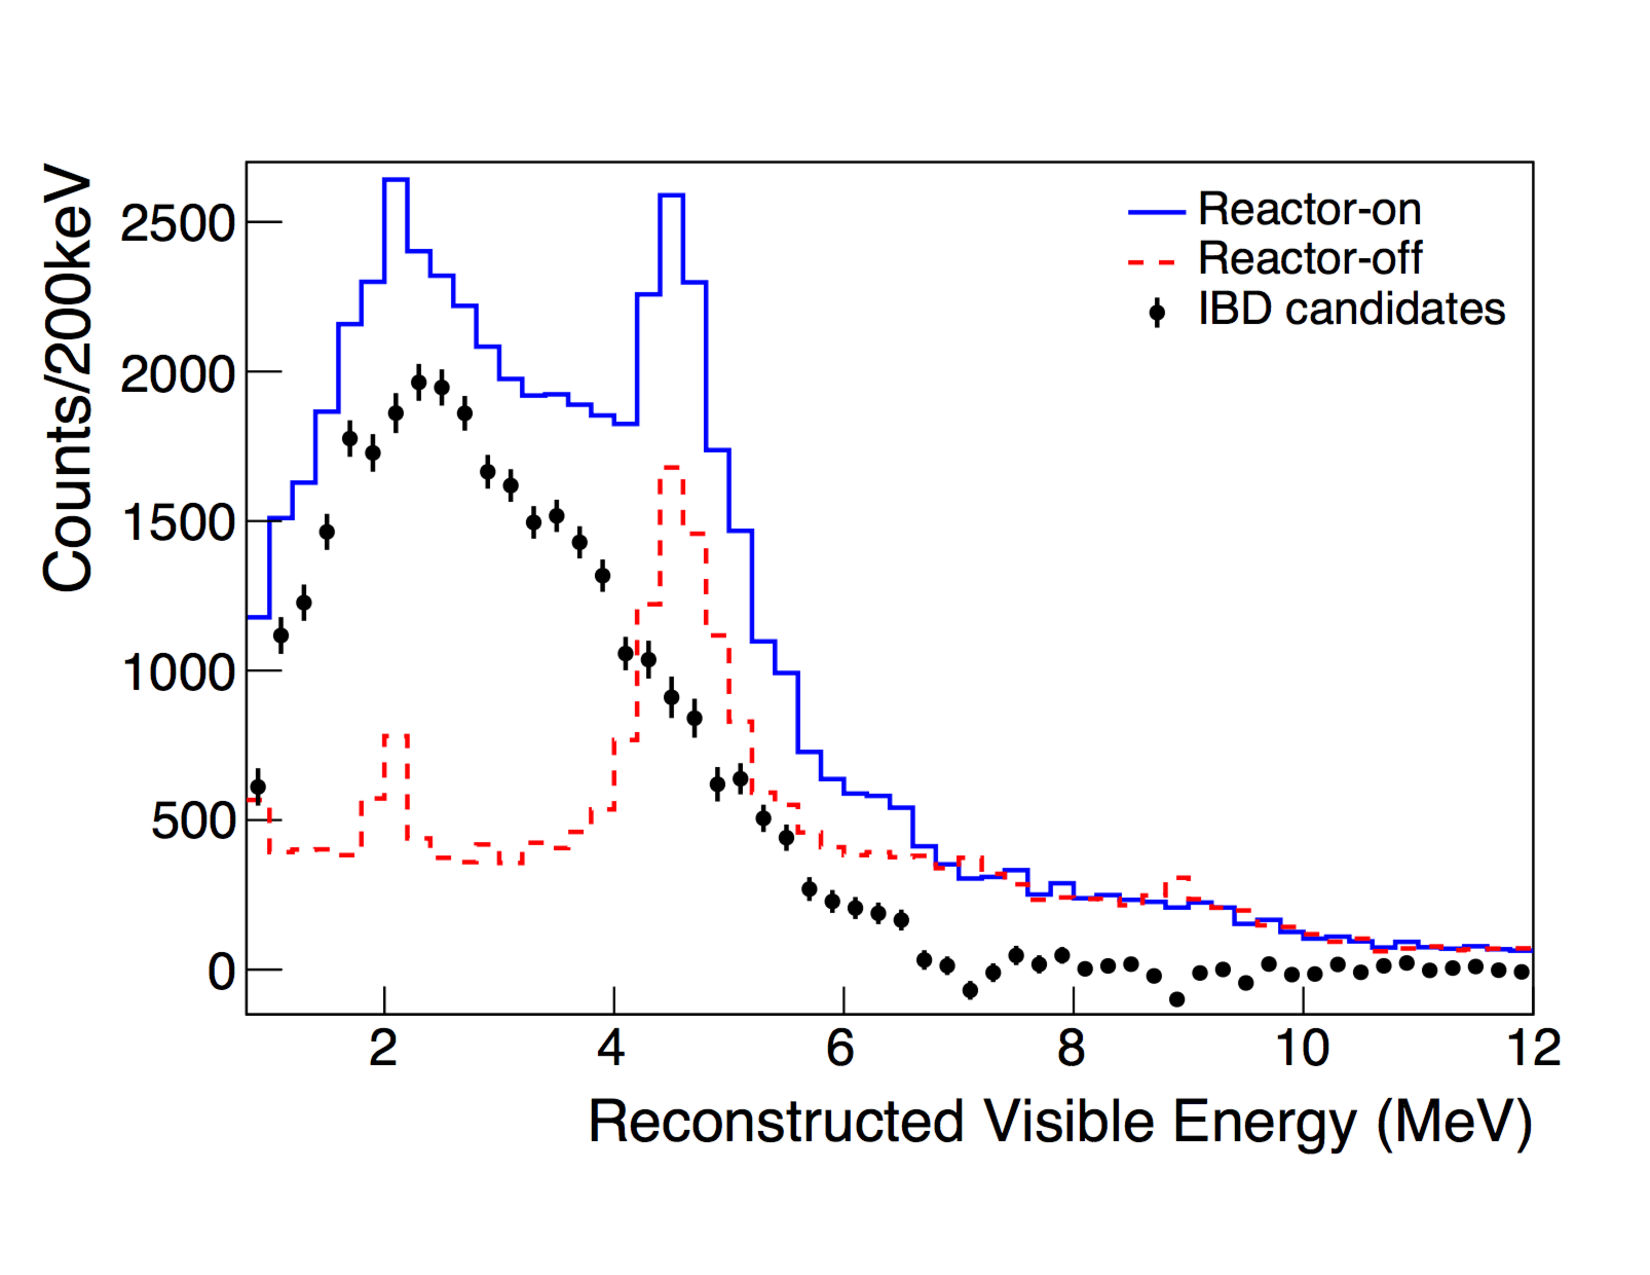
\includegraphics[width=0.8\linewidth]{tex/7-oscillation-images/Spectrum}
	\caption{Reconstructed visible prompt energy of IBD events (black), along with correlated IBD candidates in reactor on (blue, solid) and reactor off (red, dashed) periods. Errors are statistical. The reactor off spectrum has been scaled by the relative exposure time between on and off. \cite{Ashenfelter:2018jrx}}
	\label{fig:spectrumresults}
\end{figure}



